\documentclass[11pt,oneside]{article}
\usepackage[a4paper,margin=27mm,headheight=15pt]{geometry}
\usepackage[T1]{fontenc}
\usepackage[utf8]{inputenc}
\IfFileExists{libertinus.sty}{\usepackage{libertinus}}{\usepackage{lmodern}}
\usepackage{microtype}
\usepackage{amsmath,amssymb,amsthm,mathtools,mathrsfs}
\usepackage{bm}
\usepackage{booktabs,longtable,array,tabularx,multirow}
\usepackage{graphicx}
\usepackage{xcolor}
\usepackage{enumitem}
\usepackage{fancyhdr}
\usepackage{titlesec}
\usepackage{listings}
\usepackage{xurl}
\usepackage{hyperref}
\usepackage[nameinlink,noabbrev]{cleveref}
\definecolor{linkblue}{RGB}{25,75,135}
\definecolor{shadegray}{RGB}{246,247,249}
\definecolor{rulegray}{RGB}{195,201,208}
\hypersetup{
  colorlinks=true,
  linkcolor=linkblue,
  citecolor=linkblue,
  urlcolor=linkblue,
  pdftitle={Finite-Block Calculus for the Fabius--Rvachev--Thue--Morse System},
  pdfsubject={New zeta--Lambert tails, q-binomial acceleration, probabilistic deconvolution, and Lambert-W truncation laws},
  pdfkeywords={Fabius function, Rvachev up-function, Thue-Morse, q-binomial, sinc product, Lambert W, zeta, Richardson extrapolation}
}
\pagestyle{fancy}
\fancyhf{}
\fancyhead[L]{\small Fabius--Rvachev frontier results}
\fancyhead[R]{\small\nouppercase{\leftmark}}
\fancyfoot[C]{\thepage}
\renewcommand{\headrulewidth}{0.4pt}
\titleformat{\section}{\Large\bfseries}{\thesection}{0.7em}{}
\titleformat{\subsection}{\large\bfseries}{\thesubsection}{0.7em}{}
\titleformat{\subsubsection}{\normalsize\bfseries}{\thesubsubsection}{0.7em}{}
\setcounter{secnumdepth}{3}
\setcounter{tocdepth}{2}
\setlist[itemize]{leftmargin=2em,itemsep=0.25em,topsep=0.4em}
\setlist[enumerate]{leftmargin=2.3em,itemsep=0.25em,topsep=0.4em}
\setlength{\emergencystretch}{3em}
\allowdisplaybreaks[2]
\numberwithin{equation}{section}

\newtheorem{theorem}{Theorem}[section]
\newtheorem{proposition}[theorem]{Proposition}
\newtheorem{lemma}[theorem]{Lemma}
\newtheorem{corollary}[theorem]{Corollary}
\newtheorem{identity}[theorem]{Identity}
\newtheorem{conjecture}[theorem]{Conjecture}
\theoremstyle{definition}
\newtheorem{definition}[theorem]{Definition}
\newtheorem{algorithm}[theorem]{Algorithm}
\newtheorem{example}[theorem]{Example}
\newtheorem{obligation}[theorem]{Formalization obligation}
\theoremstyle{remark}
\newtheorem{remark}[theorem]{Remark}
\newtheorem{warning}[theorem]{Warning}

\newcommand{\R}{\mathbb R}
\newcommand{\C}{\mathbb C}
\newcommand{\Q}{\mathbb Q}
\newcommand{\N}{\mathbb N}
\newcommand{\Z}{\mathbb Z}
\newcommand{\E}{\mathbb E}
\newcommand{\Prob}{\mathbb P}
\newcommand{\Var}{\operatorname{Var}}
\newcommand{\Up}{\operatorname{up}}
\newcommand{\sinc}{\operatorname{sinc}}
\newcommand{\e}{\mathrm e}
\newcommand{\ii}{\mathrm i}
\newcommand{\dd}{\,\mathrm d}
\newcommand{\bigO}{\mathcal O}
\newcommand{\smallo}{o}
\newcommand{\supp}{\operatorname{supp}}
\newcommand{\eps}{\varepsilon}
\newcommand{\wt}{s_2}
\newcommand{\LambertW}{W}
\newcommand{\qbinom}[3]{\genfrac{[}{]}{0pt}{}{#1}{#2}_{#3}}
\newcommand{\fall}[2]{#1^{\underline{#2}}}
\newcommand{\repo}{\nolinkurl{Analysis/FabiusFunction}}
\newcommand{\lean}[1]{%
  \ifmmode\text{\texttt{\detokenize{#1}}}\else\nolinkurl{#1}\fi}
\newcommand{\newresult}{\textbf{Result derived in this report.}}
\newcommand{\corpusresult}{\textbf{Established in the inspected corpus.}}
\newcommand{\checked}{\textbf{Numerically cross-checked.}}

\newenvironment{proofidea}{\par\smallskip\noindent\textit{Proof architecture.}\ }{\hfill$\square$\par\smallskip}
\newenvironment{boxedremark}{%
  \par\smallskip\noindent\begin{center}\begin{minipage}{0.94\textwidth}%
  \color{black}\hrule\vspace{0.6em}\small
}{%
  \vspace{0.6em}\hrule\end{minipage}\end{center}\smallskip
}
\lstdefinestyle{pseudo}{
  basicstyle=\ttfamily\small,
  backgroundcolor=\color{shadegray},
  frame=single,
  rulecolor=\color{rulegray},
  columns=fullflexible,
  keepspaces=true,
  showstringspaces=false,
  breaklines=true,
  xleftmargin=0.7em,
  xrightmargin=0.7em,
  aboveskip=0.8em,
  belowskip=0.8em
}

\title{\bfseries A Finite-Block Calculus for the\\ Fabius--Rvachev--Thue--Morse System\\[0.4em]
\large New zeta--Lambert tails, $q$-binomial acceleration, probabilistic deconvolution, and Lambert-$W$ truncation laws}
\author{Frontier research report prepared from the complete documentation corpus\\
\small Vladimir Reshetnikov's \texttt{ProveIt} repository}
\date{27 August 2026\\
\small Corpus snapshot: living documents on \texttt{main}; frozen historical variants deduplicated through the archive provenance map}

\begin{document}
\maketitle

\begin{abstract}
The documentation tree under \repo{} already contains an unusually broad and internally
cross-checked theory of the Thue--Morse sequence, the bounded Fabius distribution function,
Rvachev's compactly supported up-function, dyadic $q$-binomial arithmetic, infinite sinc
products, and the lower-Lambert endpoint phase.  This report audits the living manuscripts,
the imported primary literature, the active Fourier-decay drafts, and the frozen historical
variants, then develops a new finite-block calculus that joins several strands which had
previously remained adjacent rather than identical.

The central observation is exact.  A single length-$2^m$ signed Thue--Morse block polynomial,
under an oscillatory substitution, is a phase-and-scale normalization of the first $m$ factors
of the Fourier sinc product; under a decaying substitution, the same polynomial is a
normalization of the first $m$ factors of the negative-Laplace product used in endpoint
asymptotics.  The omitted tail is not merely small: it is a scaled copy of the full product.
This yields (i) a convergent all-orders expansion whose coefficients are zeta values arranged
as a Lambert series with base $q=1/4$; (ii) explicit, sharp-radius remainder bounds;
(iii) arbitrary-order finite Thue--Morse approximants to the Fourier transform; (iv) a
$q$-binomial Richardson scheme whose order-$p$ extrapolant converges like
$4^{-(p+1)m}$; (v) an exact random-tail decomposition and a weak differential expansion of
the up-density in terms of finite uniform splines; (vi) a Lambert-$W$ law for the number of
product factors needed on the canonical endpoint saddle scale; and (vii) a Barnes-like tower
built from derivatives of the entire shifted Thue--Morse Dirichlet function at its trivial
zeros.

All stated theorems are proved here.  High-precision computations independently check the
finite identities, coefficients, asymptotic orders, and truncation laws.  The phrase
``new result'' means new to the inspected repository corpus and derived in this report; no
claim of global publication priority is made without a dedicated literature review beyond
the searches recorded here.
\end{abstract}

\begin{boxedremark}
\textbf{Status discipline.}
The report uses three levels.  Statements explicitly attributed to the repository or to the
literature are background.  Statements labeled ``Result derived in this report'' are supplied
with proofs.  Numerical experiments are validation, not substitutes for proof.  Several final
research directions are labeled as conjectures or formalization obligations.

\smallskip
\textbf{Formalization crosswalk.}
``Result derived in this report'' is a statement about the inspected \emph{prose} corpus and
says nothing about the Lean library.  In fact several of the results below already have formal
counterparts in \nolinkurl{Analysis/FabiusFunction/Lean/FabiusFunction/}, in some cases proved
there in greater generality than they are stated here.  Wherever this is so, a paragraph
headed \emph{Formal version} follows the statement and gives the exact declaration names,
typeset as \lean{Fabius.thueMorseSign}, together with the module they live in; where the Lean
statement is weaker (real argument only, or the identity before a normalization) or stronger
(arbitrary ring, arbitrary base, arbitrary interpolation ratio) than the statement here, the
paragraph says which.  Absence of such a paragraph means only that no formal counterpart was
located, and must not be read as a claim that none exists.  A paper proof is in any case not
evidence of formalization, and a citation to a more general Lean theorem is not a claim that
the exact statement printed here has been formalized.
\end{boxedremark}

\tableofcontents
\clearpage

\section{Corpus audit and research positioning}
\label{sec:audit}

\subsection{What was inspected}

The repository's documentation is not one article but a layered research environment.  The
living primary exposition separates the bounded cumulative distribution $F$, the even bump
$\Up$, and the signed global extension, and develops their construction, probability model,
Fourier products, dyadic arithmetic, and corrected endpoint asymptotics.  The consolidated
frontier volume records non-formalized deductions and gaps; the Thue--Morse Atlas develops a
large formula network; the active Fourier-decay directory contains twelve mutually auditing
manuscripts; the non-elementarity article and Lean walkthrough provide logical and formal
context; and the papers directory contains source TeX for relevant primary literature.
The archive is explicitly a provenance-preserving collection of frozen versions, with
byte-identical or otherwise redundant entries pruned from the historical catalogue
\cite{proveit-primary,proveit-frontiers,proveit-atlas,proveit-fourier,proveit-archive}.

The audit protocol was therefore:
\begin{enumerate}
\item read the current living manuscripts as the authoritative mathematical state;
\item compare the active Fourier-decay drafts because they contain genuinely different
      hypotheses, corrections, and audit conclusions;
\item inspect each imported paper represented by TeX source;
\item use the archive's commit-level provenance map to deduplicate superseded historical
      copies, while retaining every uniquely described line of development in the research map;
\item search the corpus for the candidate identities and coefficient patterns before calling
      them new to the corpus.
\end{enumerate}
A complete source ledger appears in \cref{app:ledger}.

\subsection{Established pillars}

The following table compresses the established state which this report uses but does not
re-prove in full.

\begin{center}
\small
\begin{tabularx}{\textwidth}{@{}p{0.20\textwidth}X X@{}}
\toprule
Pillar & Established content & Remaining junction exploited here \\
\midrule
Thue--Morse & $\eps_n=(-1)^{s_2(n)}$, block products, Prouhet cancellation, Mahler equations,
Walsh and lacunary products, shifted entire Dirichlet theory & Turn one finite block into a
certified approximation engine for both Fourier and Laplace products \\
Fabius/up probability & $\Up$ as a compactly supported probability density and $F$ as its
rescaled CDF; finite atomic/uniform convolution models & Identify the omitted convolution tail
as an exact scaled copy and expand it to all orders \\
Fourier analysis & $\widehat{\Up}$ as a dyadic sinc product; shell factorization; pointwise,
metric, averaged, and extremal decay regimes & Analyze truncation in the small tail variable,
which is complementary to large-frequency shell dynamics \\
Dyadic arithmetic & exact values at dyadic rationals, $q$-Pochhammer and Gaussian-binomial
formulae at base $1/2$, Thue--Morse coefficient extraction & Produce a new Gaussian-binomial
role at base $q=1/4$: geometric-grid extrapolation weights \\
Endpoint asymptotics & negative-Laplace product, periodic lower-Lambert phase, all-orders saddle
expansion, $\lambda=-W_{-1}(-x\log2)/\log2$ & Quantify the finite-product depth on the canonical
Lambert scale and express it through one finite Thue--Morse block \\
Formalization & extensive Lean construction and exact proof correspondence; explicit quarantine
of unformalized claims & Isolate short algebraic and analytic lemmas suitable for promotion \\
\bottomrule
\end{tabularx}
\end{center}

\subsection{The missing commutative bridge}

The corpus contains all four vertices of the following conceptual square:
\[
\begin{array}{ccc}
\text{finite Thue--Morse blocks} & \longrightarrow & \text{finite dyadic products}\\
\Big\downarrow && \Big\downarrow\\
\text{exact dyadic arithmetic} & \longrightarrow & \text{Fourier/Laplace asymptotics}.
\end{array}
\]
What was not isolated as one theorem package is that the top horizontal arrow has two exact
specializations, oscillatory and decaying, and that the right vertical arrow has a
self-similar tail with an analytic expansion in the geometric parameter $4^{-m}$.  Once this
is written down, zeta values, Lambert series, Gaussian binomials, random-tail moments, and the
Lambert-$W$ endpoint phase become parts of one finite-block calculus rather than separate
phenomena.

\subsection{Priority and uncertainty}

Keyword searches of the inspected TeX corpus did not locate the all-orders $4^{-m}$ tail
formula, the sharp-radius remainder bound, or the $q$-binomial extrapolation scheme in the
form proved below.  Searches of arXiv and publisher records located the classical Fabius,
Thue--Morse, lacunary-product, automatic-sequence, arithmetic, Dirichlet-series, and
Lambert-$W$ sources used for context \cite{arias1982,arias2017arith,aistleitner2015,
toth2022,corless1996,allouche2003}, but did not constitute an exhaustive priority search.  Accordingly, every novelty statement in this report is
corpus-relative.

\section{Objects, normalizations, and exact background}
\label{sec:objects}

\subsection{The signed block polynomial}

Let
\begin{equation}
 \eps_n=(-1)^{s_2(n)},\qquad
 P_m(z)=\sum_{n=0}^{2^m-1}\eps_n z^n
       =\prod_{j=0}^{m-1}\left(1-z^{2^j}\right),
 \label{eq:Pm}
\end{equation}
where $s_2(n)$ is the binary digit sum.  The product identity is the finite form of the
Thue--Morse generating-product law.  Its zero of order $m$ at $z=1$ is exactly the Prouhet
cancellation of moments of degrees below $m$.

\emph{Formal version.}  The product identity in \eqref{eq:Pm} is
\lean{Fabius.prod_one_sub_pow_eq_sum_thueMorseSign} (\path{ThueMorseBooleanCube.lean}),
which is more general than the form used here: it is stated for $z$ in an arbitrary
commutative ring, not for complex $z$, and is proved once by a Boolean-cube expansion.  Every
substitution made below --- $z=\e^{\ii t/2^{m-1}}$ in \cref{thm:finite-sinc},
$z=\e^{-s/2^m}$ in \cref{thm:finite-Laplace} --- is an instance of that single statement.

\subsection{Fourier and Laplace products}

Use $\sinc z=\sin z/z$ with $\sinc0=1$, and define
\begin{align}
 Q_m(t)&=\prod_{k=1}^{m}\sinc\!\left(\frac{t}{2^k}\right),
 &Q_\infty(t)&=\prod_{k=1}^{\infty}\sinc\!\left(\frac{t}{2^k}\right),
 \label{eq:Qdef}\\
 G_m(-s)&=\prod_{k=1}^{m}\frac{1-\e^{-s/2^k}}{s/2^k},
 &G(-s)&=\prod_{k=1}^{\infty}\frac{1-\e^{-s/2^k}}{s/2^k}.
 \label{eq:Gdef}
\end{align}
The products converge locally uniformly and define entire functions after removable values
at zero are supplied.

With the Fourier convention
\[
 \widehat h(\xi)=\int_{\R}h(x)\e^{-2\pi\ii x\xi}\dd x,
\]
the normalized Rvachev density satisfies
\begin{equation}
 \widehat{\Up}(\xi)=Q_\infty(2\pi\xi)
 =\prod_{j=0}^{\infty}\sinc\!\left(\frac{\pi\xi}{2^j}\right).
 \label{eq:upFourier}
\end{equation}
The bounded Fabius distribution is related by
\begin{equation}
 F'(x)=2\Up(2x-1),\qquad
 F(x)=\int_{-1}^{2x-1}\Up(y)\dd y\quad(0\le x\le1).
 \label{eq:Fup}
\end{equation}
These conventions agree with the repository's primary exposition
\cite{proveit-primary,arias1982}.

\emph{Formal versions, and the convention check.}  Both normalizations used above are the ones
carried by the Lean library, which matters because the corpus contains more than one Fourier
convention and a crosswalk across a mismatch would be worthless.  The Lean transform
\lean{Fabius.rvachevFourier} is defined as $\int_\R\Up(t)\e^{-2\pi\ii tz}\dd t$ --- the
convention of \eqref{eq:upFourier} --- and
\lean{Fabius.rvachevFourier_eq_product} (\path{FourierProduct.lean}) proves it equal to
\lean{Fabius.rvachevFourierProduct}, namely $\prod_{n\ge0}\sinc(\pi z/2^n)$.  That is
\eqref{eq:upFourier} verbatim.  Likewise $G$ in \eqref{eq:Gdef} is the Lean object
\lean{Fabius.complexGeneratingFunction}: that the entire half-moment generating function
evaluated at $-s$ equals the dyadic product $\prod_{k\ge1}(1-\e^{-s/2^k})/(s/2^k)$ of
\eqref{eq:Gdef}, with the same removable value at each vanishing factor, is
\lean{Fabius.complexGeneratingFunction_neg_eq_tprod}
(\path{NegativeLaplaceVertical.lean}), for every $s\in\C$.

\subsection{The lower-Lambert phase}

Write $L=\log2$.  For small $x>0$, the canonical endpoint phase variable is
\begin{equation}
 \lambda(x)=-\frac{W_{-1}(-Lx)}{L},
 \qquad x=\lambda(x)2^{-\lambda(x)}.
 \label{eq:lambda}
\end{equation}
The associated leading saddle scale is
\begin{equation}
 s_0(x)=2^{\lambda(x)}=\frac{\lambda(x)}{x}.
 \label{eq:s0}
\end{equation}
The repository's endpoint theory adds periodic corrections in $\log_2s$ and an all-orders
saddle expansion.  Our use of \eqref{eq:s0} below is computational: it measures how many
factors of the exact product are needed near that scale.  It is not a replacement for the
periodically corrected saddle analysis.

\section{One Thue--Morse block, two exact product bridges}
\label{sec:bridges}

\subsection{Oscillatory specialization: the Fourier bridge}

\begin{theorem}[Exact finite Thue--Morse--sinc identity]
\label{thm:finite-sinc}
For every integer $m\ge1$ and every $t\in\C$,
\begin{equation}
 \boxed{
 P_m\!\left(\e^{\ii t/2^{m-1}}\right)
 =(-\ii)^m t^m 2^{-\binom m2}
   \e^{\ii t(1-2^{-m})}Q_m(t).}
 \label{eq:finite-sinc}
\end{equation}
Equivalently, with the removable value at $t=0$ understood,
\begin{equation}
 \boxed{
 Q_m(t)=\ii^m2^{\binom m2}t^{-m}
 \e^{-\ii t(1-2^{-m})}
 \sum_{n=0}^{2^m-1}\eps_n\e^{\ii nt/2^{m-1}}.}
 \label{eq:normalized-TM-Fourier}
\end{equation}
\newresult
\end{theorem}

\begin{proof}
Insert $z=\e^{\ii t/2^{m-1}}$ in the product form of $P_m$ and reverse the
index:
\[
 P_m(z)=\prod_{k=0}^{m-1}\left(1-\e^{\ii t/2^k}\right).
\]
For each factor use
\[
 1-\e^{\ii x}=(-\ii)x\e^{\ii x/2}\sinc(x/2).
\]
The product of the linear terms is
\[
 (-\ii)^m t^m2^{-\sum_{k=0}^{m-1}k}
 =(-\ii)^m t^m2^{-\binom m2}.
\]
The product of the phases is
\[
 \exp\!\left(\frac{\ii t}{2}\sum_{k=0}^{m-1}2^{-k}\right)
 =\e^{\ii t(1-2^{-m})},
\]
and the sinc factors are $\sinc(t/2),\ldots,\sinc(t/2^m)$.  This gives
\eqref{eq:finite-sinc}; the sum form follows from \eqref{eq:Pm}.
\end{proof}

\emph{Formal version.}  The unnormalized half of \eqref{eq:finite-sinc} is
\lean{Fabius.sum_thueMorseSign_exp_eq_sin_prod} (\path{ThueMorseSineProduct.lean}), which
states, for real $x$ and every $m$,
\[
 \sum_{n<2^m}\eps_n\e^{\ii nx}
 =(-2\ii)^m\e^{\ii(2^m-1)x/2}\prod_{j<m}\sin\!\left(\frac{2^jx}{2}\right),
\]
the half-angle factorization $1-\e^{\ii v}=-2\ii\,\e^{\ii v/2}\sin(v/2)$ being isolated as
\lean{Fabius.one_sub_exp_mul_I}.  Setting $x=t/2^{m-1}$ and extracting the linear factor from
each $\sin(t/2^k)$ turns it into \eqref{eq:finite-sinc}.  The Lean statement is therefore this
theorem before the $\sinc$ normalization, and only for real $t$; the removable value at $t=0$
and the extension to complex $t$ are not part of it.

\begin{remark}[Prouhet cancellation becomes the normalization]
The factor $t^{-m}$ in \eqref{eq:normalized-TM-Fourier} is harmless precisely because
$P_m$ has a zero of order $m$ at $1$.  Thus the same cancellation that annihilates the first
$m$ power moments also regularizes the Fourier approximation at the origin.
\end{remark}

\subsection{Decaying specialization: the endpoint Laplace bridge}

\begin{theorem}[Exact finite Thue--Morse--Laplace identity]
\label{thm:finite-Laplace}
For every integer $m\ge1$ and every $s\in\C$,
\begin{equation}
 \boxed{
 G_m(-s)=\frac{2^{m(m+1)/2}}{s^m}
 P_m\!\left(\e^{-s/2^m}\right)
 =\frac{2^{m(m+1)/2}}{s^m}
  \sum_{n=0}^{2^m-1}\eps_n\e^{-ns/2^m}.}
 \label{eq:finite-Laplace}
\end{equation}
Again, the apparent singularity at $s=0$ is removable.
\newresult
\end{theorem}

\begin{proof}
The substitution $z=\e^{-s/2^m}$ gives
\[
 P_m(z)=\prod_{j=0}^{m-1}\left(1-\e^{-s2^j/2^m}\right)
       =\prod_{k=1}^{m}\left(1-\e^{-s/2^k}\right).
\]
The denominator in $G_m(-s)$ is
\[
 \prod_{k=1}^{m}\frac{s}{2^k}
 =s^m2^{-m(m+1)/2},
\]
which proves the identity.
\end{proof}

\emph{Formal version.}  The block identity underlying \eqref{eq:finite-Laplace} is
\lean{Fabius.sum_range_two_pow_thueMorseSign_exp} (\path{ThueMorseInfiniteProduct.lean}):
\[
 \sum_{n<2^m}\eps_n\e^{-nt}=\prod_{j<m}\left(1-\e^{-2^jt}\right)
\]
for every real $t$ and every $m$, with no convergence hypothesis.  At $t=s/2^m$ this is the
content of \eqref{eq:finite-Laplace} \emph{before} division by
$\prod_{k\le m}(s/2^k)$: the normalizing factor $2^{m(m+1)/2}s^{-m}$, the removable
singularity at $s=0$, and the passage to complex $s$ are not part of the Lean statement.

\begin{boxedremark}
\textbf{The exact finite-block principle.}
The oscillatory sample $z=\e^{\ii t/2^{m-1}}$ converts $P_m$ into the truncated Fourier
product $Q_m(t)$.  The decaying sample $z=\e^{-s/2^m}$ converts the same $P_m$ into the
truncated negative-Laplace product $G_m(-s)$.  No asymptotic argument is involved.
\end{boxedremark}

\subsection{The omitted tail is a scaled copy of the whole}

\begin{proposition}[Exact tail self-similarity]
\label{prop:tail-self}
For every $m\ge0$,
\begin{align}
 Q_\infty(t)&=Q_m(t)Q_\infty(t/2^m),
 \label{eq:Q-tail-self}\\
 G(-s)&=G_m(-s)G(-s/2^m).
 \label{eq:G-tail-self}
\end{align}
\newresult
\end{proposition}

\begin{proof}
After removing the first $m$ factors, replace $k$ by $m+\ell$ in the remaining infinite
product.  The residual factors are exactly those of the original product evaluated at the
scaled argument.
\end{proof}

\emph{Formal versions.}  Both halves are formalized, and the first is formalized in a form
strictly more general than the one stated here.  The reindexing itself is
\lean{Fabius.tprod_geom_scale_pow} (\path{GeometricScaleProducts.lean}): for an arbitrary
function $g$ from a field into a commutative topological monoid, an arbitrary nonzero scale
$c$, and every $k$,
\[
 \prod_{n\ge0}g\!\left(\frac{c^kz}{c^n}\right)
 =\left(\prod_{j<k}g\!\left(c^{j+1}z\right)\right)\prod_{n\ge0}g\!\left(\frac{z}{c^n}\right),
\]
the only hypothesis being multipliability of the undilated family; nothing about $\sinc$,
about base two, or even about $\C$ enters, and $g=\sinc$, $c=2$, $z=t/2^{m+1}$, $k=m$ gives
\eqref{eq:Q-tail-self}.  The instance stated directly for the transform is
\lean{Fabius.rvachevFourier_eq_finite_product} (\path{FourierProduct.lean}), in the
$\e^{-2\pi\ii x\xi}$ convention of \eqref{eq:upFourier}.  The Laplace half
\eqref{eq:G-tail-self} is \lean{Fabius.complexGeneratingFunction_neg_finite_refinement}
(\path{NegativeLaplaceVertical.lean}), an exact identity for every $m$ and every $s\in\C$.

\begin{corollary}[Exact finite Thue--Morse factorization of the full products]
\label{cor:full-TM-factor}
For $m\ge1$,
\begin{align}
 Q_\infty(t)
 &=\ii^m2^{\binom m2}t^{-m}\e^{-\ii t(1-2^{-m})}
   P_m\!\left(\e^{\ii t/2^{m-1}}\right)Q_\infty(t/2^m),
 \label{eq:full-Q-TM}\\
 G(-s)
 &=\frac{2^{m(m+1)/2}}{s^m}
   P_m\!\left(\e^{-s/2^m}\right)G(-s/2^m).
 \label{eq:full-G-TM}
\end{align}
Thus every truncation error is represented by the original entire function in a small
argument.
\end{corollary}

\section{The zeta--Lambert tail calculus}
\label{sec:zeta-tail}

\subsection{A local logarithm of the sinc function}

\begin{lemma}[Euler--zeta expansion]
\label{lem:logsinc}
For $|z|<\pi$,
\begin{equation}
 \boxed{
 \log\sinc z
 =-\sum_{r=1}^{\infty}\frac{\zeta(2r)}{r\pi^{2r}}z^{2r}.}
 \label{eq:logsinc}
\end{equation}
The logarithm is the branch vanishing at $z=0$.
\end{lemma}

\begin{proof}
Euler's product gives
\[
 \frac{\sin z}{z}=\prod_{n=1}^{\infty}
 \left(1-\frac{z^2}{\pi^2n^2}\right).
\]
For $|z|<\pi$, expand $\log(1-w)=-\sum_{r\ge1}w^r/r$.  Absolute local uniform
convergence permits interchanging the sums, and the inner sum over $n$ is $\zeta(2r)$.
\end{proof}

\emph{Formal versions.}  The branch-free content of \eqref{eq:logsinc} is formalized in
\path{SincZetaSeries.lean} as the exponential identity
\lean{Fabius.complexSinc\_pi\_mul\_eq\_cexp}: for complex $x$ with $|x|<1$,
$\sinc(\pi x)=\exp\bigl(-\sum_{r\ge1}\zeta(2r)x^{2r}/r\bigr)$, the values $\zeta(2r)$ carried
as the elementary series \lean{Fabius.evenZeta} (\path{EvenZetaSeries.lean}); the $|z|<\pi$
normalization printed above is \lean{Fabius.complexSinc\_eq\_cexp}.  For real $0<|x|<1$ the
boxed logarithmic form itself is \lean{Fabius.log\_sin\_div\_pi\_mul}, the branch being the
real logarithm --- exactly the branch vanishing at $0$.  The interchange of sums is performed
once, in greater generality than this lemma needs (an arbitrary absolutely summable family
with every norm below $1$, over an arbitrary index type), by the Euler log transform
\lean{Fabius.hasSum\_powerSum\_log\_one\_sub} of \path{EulerLogTransform.lean}; the closed
evaluations $\zeta(2)=\pi^2/6$ and $\zeta(4)=\pi^4/90$ and the general Bernoulli form are
\path{EvenZetaValues.lean}.

\subsection{All orders, exact radius, explicit remainder}

\begin{theorem}[All-orders sinc-tail expansion]
\label{thm:all-orders-Q}
Let $m\ge0$.  For
\begin{equation}
 |t|<\pi2^{m+1},
 \label{eq:Q-domain}
\end{equation}
the quotient $Q_\infty(t)/Q_m(t)$ is nonzero and
\begin{equation}
 \boxed{
 \log\frac{Q_\infty(t)}{Q_m(t)}
 =-\sum_{r=1}^{\infty}
 \frac{\zeta(2r)}{r\pi^{2r}(4^r-1)}
 t^{2r}4^{-rm}.}
 \label{eq:Q-all-orders}
\end{equation}
The disk in \eqref{eq:Q-domain} is maximal for this Taylor logarithm: its boundary contains
the nearest zeros $t=\pm\pi2^{m+1}$ of the tail.
\newresult
\end{theorem}

\begin{proof}
By \cref{prop:tail-self}, the quotient is $Q_\infty(t/2^m)$.  Apply
\cref{lem:logsinc} to every factor and sum:
\begin{align*}
 \log Q_\infty(t/2^m)
 &=-\sum_{k=1}^{\infty}\sum_{r=1}^{\infty}
   \frac{\zeta(2r)}{r\pi^{2r}}
   \left(\frac{t}{2^{m+k}}\right)^{2r}\\
 &=-\sum_{r=1}^{\infty}\frac{\zeta(2r)t^{2r}}{r\pi^{2r}}
   \frac{4^{-r(m+1)}}{1-4^{-r}}\\
 &=-\sum_{r=1}^{\infty}
   \frac{\zeta(2r)}{r\pi^{2r}(4^r-1)}t^{2r}4^{-rm}.
\end{align*}
The closest zero of $Q_\infty(w)$ to $w=0$ is $w=\pm2\pi$, arising from the factor
$\sinc(w/2)$.  Scaling by $w=t/2^m$ proves maximality.
\end{proof}

\emph{Formal versions.}  The theorem is formalized in \path{SincZetaDyadic.lean}, in the
normalization $\Phi(z)=Q_\infty(2\pi z)$ and in exponential form.  At $m=0$,
\lean{Fabius.rvachevFourierProduct\_eq\_cexp} proves
$\Phi(z)=\exp\bigl(-\sum_{r\ge1}\zeta(2r)4^rz^{2r}/(r(4^r-1))\bigr)$ on $|z|<1$; for general
$m$, \lean{Fabius.rvachevFourierProduct\_eq\_prefix\_mul\_cexp} is the exact factorization
$\Phi(z)=\bigl(\prod_{j<m}\sinc(\pi z/2^j)\bigr)\exp\bigl(-\sum_{r\ge1}
\zeta(2r)4^r(z/2^m)^{2r}/(r(4^r-1))\bigr)$ on $|z|<2^m$ --- identity \eqref{eq:Q-all-orders}
with the quotient cleared and the finite prefix explicit.  The engine is one application of
the Euler log transform to the pair family $(z/2^h)^2/(n+1)^2$ over $\N\times\N$; its power
sums are evaluated for \emph{every} complex $z$, with no smallness hypothesis
(\lean{Fabius.sinc\_pair\_powerSum}).  Maximality of the disk is not formalized.

The first terms are
\begin{equation}
 \frac{Q_\infty(t)}{Q_m(t)}
 =\exp\!\left(
 -\frac{t^2}{18}4^{-m}
 -\frac{t^4}{2700}16^{-m}
 -\frac{t^6}{178605}64^{-m}
 -\frac{t^8}{9639000}256^{-m}
 -\cdots\right).
 \label{eq:Q-first-terms}
\end{equation}

\begin{theorem}[Certified tail remainder]
\label{thm:Q-remainder}
Let $N\ge0$ and put
\begin{equation}
 x_m(t)=\frac{|t|}{\pi2^{m+1}}<1.
 \label{eq:xmt}
\end{equation}
If $R_{N,m}(t)$ denotes the part of the positive series in
\eqref{eq:Q-all-orders} with $r\ge N+1$, then
\begin{equation}
 \boxed{
 |R_{N,m}(t)|
 \le \frac{4\zeta(2)}{3}
 \frac{x_m(t)^{2N+2}}{(N+1)(1-x_m(t)^2)}.}
 \label{eq:Q-remainder-bound}
\end{equation}
For real $t$ in the stated disk, $R_{N,m}(t)\ge0$.
\newresult
\end{theorem}

\begin{proof}
Rewrite the absolute value of the $r$-th term as
\[
 \frac{\zeta(2r)}{r}\frac{4^r}{4^r-1}x_m(t)^{2r}.
\]
Use $\zeta(2r)\le\zeta(2)$, $4^r/(4^r-1)\le4/3$, and
$1/r\le1/(N+1)$ for $r\ge N+1$, then sum the geometric series.
\end{proof}

\emph{Formal versions.}  \path{SincZetaRemainder.lean} packages the coefficient as
\lean{Fabius.sincZetaCoeff} and proves \eqref{eq:Q-remainder-bound} verbatim as
\lean{Fabius.norm\_sincZeta\_tail\_le}, with $x_m(t)=\|w\|$ for $w=z/2^m$, alongside the
term-by-term nonnegativity for real arguments (\lean{Fabius.sincZeta\_tail\_nonneg}) and the
three-factor coefficient estimate of this proof
(\lean{Fabius.sincZetaCoeff\_le}, resting on the antitonicity
\lean{Fabius.evenZeta\_anti} of the even zeta values).  The constant is carried symbolically
as $\tfrac43\zeta(2)$; the numerical value $2\pi^2/9$ follows from
\lean{Fabius.evenZeta\_one} (\path{EvenZetaValues.lean}).

\subsection{Arbitrary-order finite Thue--Morse approximants}

\begin{definition}[Zeta-corrected block approximant]
For $N\ge0$ define
\begin{equation}
 Q_m^{[N]}(t)=Q_m(t)
 \exp\!\left[-\sum_{r=1}^{N}
 \frac{\zeta(2r)t^{2r}}{r\pi^{2r}(4^r-1)}4^{-rm}\right].
 \label{eq:Qcorrected}
\end{equation}
For $N=0$, this is $Q_m$.
\end{definition}

\begin{corollary}[Arbitrary-order convergence]
\label{cor:arbitrary-Q}
For every compact set $K\subset\C$ and every fixed $N\ge0$,
\begin{equation}
 Q_m^{[N]}(t)=Q_\infty(t)
 \left(1+\bigO_K(4^{-(N+1)m})\right)
 \qquad(t\in K,\ m\to\infty).
 \label{eq:arbitrary-Q}
\end{equation}
Moreover, after inserting \eqref{eq:normalized-TM-Fourier}, the left side is a normalized
length-$2^m$ Thue--Morse exponential sum multiplied by only $N$ explicit zeta corrections.
\newresult
\end{corollary}

\begin{proof}
For all sufficiently large $m$, $K$ lies in the disk \eqref{eq:Q-domain}.  The exact quotient
$Q_\infty/Q_m^{[N]}$ is $\exp(-R_{N,m})$.  The bound
\eqref{eq:Q-remainder-bound}, uniformly on $K$, is $\bigO_K(4^{-(N+1)m})$; exponentiation
preserves that order.
\end{proof}

\emph{Formal versions.}  The quantitative content is
\lean{Fabius.rvachevFourierProduct\_eq\_prefix\_mul\_correction\_mul\_tail}
(\path{SincZetaRemainder.lean}): on $|z|<2^m$, exactly
$\Phi(z)=\bigl(\prod_{j<m}\sinc(\pi z/2^j)\bigr)\cdot
\exp\bigl(-\sum_{r=1}^{N}c_r(z/2^m)^{2r}\bigr)\cdot\exp\bigl(-R_{N}(z/2^m)\bigr)$, the finite
prefix being the length-$2^m$ Thue--Morse block of \cref{cor:full-TM-factor}, the middle
factor the $N$ zeta corrections of \eqref{eq:Qcorrected}, and the tail exponent bounded by
\lean{Fabius.norm\_sincZeta\_tail\_le}.  The $\bigO_K$ formulation printed here is a direct
reading of that bound and is not separately formalized.

\begin{corollary}[Fourier approximation to the up-function]
\label{cor:up-Fourier-block}
For fixed $\xi\in\C$,
\begin{align}
 \widehat\Up(\xi)
 &=\ii^m2^{\binom m2}(2\pi\xi)^{-m}
   \e^{-2\pi\ii\xi(1-2^{-m})}
   \sum_{n=0}^{2^m-1}\eps_n
   \e^{2\pi\ii n\xi/2^{m-1}}
 \notag\\[-0.2em]
 &\quad\times
 \exp\!\left[-\sum_{r=1}^{N}
 \frac{\zeta(2r)(2\pi\xi)^{2r}}{r\pi^{2r}(4^r-1)}4^{-rm}\right]
 \left(1+\bigO_{\xi,N}(4^{-(N+1)m})\right).
 \label{eq:up-TM-approx}
\end{align}
Thus the infinite Fourier product admits an arbitrary-order approximation from one finite
digital block.
\end{corollary}

\subsection{Why the coefficient array is a Lambert series}

Put $q=1/4$.  Then \eqref{eq:Q-all-orders} becomes
\begin{equation}
 \log\frac{Q_\infty(t)}{Q_m(t)}
 =-\sum_{r=1}^{\infty}
 \frac{\zeta(2r)}{r\pi^{2r}}t^{2r}
 \frac{q^{r(m+1)}}{1-q^r}.
 \label{eq:Q-Lambert}
\end{equation}
The kernel $q^r/(1-q^r)$ is the elementary Lambert-series kernel.  Expanding it as
$\sum_{\ell\ge1}q^{r\ell}$ reconstructs the omitted factors.  This is a direct analytic
connection between the sinc product and $q$-series: the base is $q=1/4$ because the logarithm
is even and the geometric frequency scale is $1/2$.

The kernel itself is now formal, in a generality independent of the sinc product: for complex
$|w|<1$ and $|c|<1$, \lean{Fabius.tsum\_log\_one\_sub\_geom} (\path{EulerLogTransform.lean})
proves $\sum_{k\ge0}\log(1-wc^k)=-\sum_{r\ge1}w^r/(r(1-c^r))$, and
\lean{Fabius.tprod\_one\_sub\_geom\_eq\_cexp} is the exponential $q$-Pochhammer form
$(w;c)_\infty=\exp\bigl(-\sum_{r\ge1}w^r/(r(1-c^r))\bigr)$, with real counterparts
(\lean{Fabius.tsum\_log\_one\_sub\_geom\_real},
\lean{Fabius.tprod\_one\_sub\_geom\_eq\_rexp}).

\begin{theorem}[General geometric base]
\label{thm:base-b}
Let $b>1$ and
\[
 Q_{m,b}(t)=\prod_{k=1}^{m}\sinc(t/b^k),\qquad
 Q_{\infty,b}(t)=\prod_{k=1}^{\infty}\sinc(t/b^k),\qquad q=b^{-2}.
\]
For $|t|<\pi b^{m+1}$,
\begin{equation}
 \boxed{
 \log\frac{Q_{\infty,b}(t)}{Q_{m,b}(t)}
 =-\sum_{r=1}^{\infty}\frac{\zeta(2r)}{r\pi^{2r}}t^{2r}
 \frac{q^{r(m+1)}}{1-q^r}.}
 \label{eq:base-b}
\end{equation}
\newresult
\end{theorem}

\begin{proof}
Repeat the proof of \cref{thm:all-orders-Q}, replacing the geometric sum in $4^{-r}$ by the
one in $b^{-2r}$.
\end{proof}

\section{An all-orders finite-block formula for the endpoint Laplace product}
\label{sec:Laplace-tail}

\subsection{Centering removes the linear tail}

\begin{lemma}[Fourier--Laplace rotation]
\label{lem:GQ}
For every $s\in\C$,
\begin{equation}
 \boxed{G(-s)=\e^{-s/2}Q_\infty(\ii s/2).}
 \label{eq:GQ}
\end{equation}
More generally,
\begin{equation}
 G_m(-s)=\e^{-\frac{s}{2}(1-2^{-m})}Q_m(\ii s/2).
 \label{eq:GmQm}
\end{equation}
\end{lemma}

\begin{proof}
For every $v$,
\[
 \frac{1-\e^{-v}}{v}=\e^{-v/2}\frac{\sinh(v/2)}{v/2}
 =\e^{-v/2}\sinc(\ii v/2).
\]
Multiply with $v=s/2^k$.  The linear exponents sum to $-s/2$ in the infinite product and to
$-s(1-2^{-m})/2$ in the finite product.
\end{proof}

\emph{Formal version.}  The infinite case \eqref{eq:GQ} is formalized, as the composite of
three named theorems.  \lean{Fabius.complexGeneratingFunction_neg_eq_tprod}
(\path{NegativeLaplaceVertical.lean}) identifies $G(-s)$ with the entire half-moment
generating function, as recorded after \eqref{eq:Gdef};
\lean{Fabius.complexGeneratingFunction_eq_fourier_analytic} (\path{FourierAnalytic.lean})
states that generating function to be $\e^{z/2}\widehat\Up(\ii z/(4\pi))$ for every
$z\in\C$; and \lean{Fabius.rvachevFourier_eq_product} (\path{FourierProduct.lean}) replaces
$\widehat\Up$ by its sinc product.  Since $\widehat\Up(\ii z/(4\pi))=Q_\infty(\ii z/2)$ in the
normalization \eqref{eq:upFourier}, and $Q_\infty$ is even, the composite at $z=-s$ is exactly
\eqref{eq:GQ}.  The finite form \eqref{eq:GmQm} has no separate Lean statement.

Define the centered products
\begin{equation}
 C(-s)=\e^{s/2}G(-s),\qquad
 C_m(-s)=\e^{\frac{s}{2}(1-2^{-m})}G_m(-s).
 \label{eq:centered-G}
\end{equation}
Then $C(-s)=Q_\infty(\ii s/2)$ and
\begin{equation}
 C(-s)=C_m(-s)C(-s/2^m).
 \label{eq:centered-tail}
\end{equation}
The centering is not cosmetic: the raw tail has a first-order error, while the centered tail
has a second-order error.

\subsection{Bernoulli--zeta expansion of the negative tail}

\begin{theorem}[All-orders negative-Laplace tail]
\label{thm:G-all-orders}
For $|u|<4\pi$,
\begin{equation}
 \boxed{
 \log G(-u)
 =-\frac{u}{2}
 +\sum_{r=1}^{\infty}
 \frac{B_{2r}}{2\,r\,(2r)!\,(4^r-1)}u^{2r}.}
 \label{eq:G-all-orders}
\end{equation}
Equivalently,
\begin{equation}
 \log C(-u)
 =\frac{u^2}{72}-\frac{u^4}{43200}
  +\frac{u^6}{11430720}-\frac{u^8}{2467584000}+\cdots.
 \label{eq:C-first}
\end{equation}
The radius $4\pi$ is exact.
\newresult
\end{theorem}

\begin{proof}
Use \cref{lem:GQ} and \cref{thm:all-orders-Q} with $m=0$ and $t=\ii u/2$:
\[
 \log G(-u)=-\frac u2
 -\sum_{r\ge1}\frac{\zeta(2r)}{r\pi^{2r}(4^r-1)}
 (-1)^r\frac{u^{2r}}{4^r}.
\]
The standard evaluation
\[
 \zeta(2r)=(-1)^{r+1}\frac{B_{2r}(2\pi)^{2r}}{2(2r)!}
\]
reduces the coefficient to the one displayed.  The closest zeros of $G(-u)$ are
$u=\pm4\pi\ii$, coming from $1-\e^{-u/2}$, so the logarithmic radius is exact.
\end{proof}

\begin{corollary}[Certified remainder for the centered Laplace tail]
\label{cor:G-remainder}
Let $y=|u|/(4\pi)<1$.  If the series in \eqref{eq:G-all-orders} is stopped after $u^{2N}$,
while the exact linear term $-u/2$ is retained, then the remainder $\mathcal R_N(u)$ obeys
\begin{equation}
 |\mathcal R_N(u)|
 \le \frac{4\zeta(2)}{3}
 \frac{y^{2N+2}}{(N+1)(1-y^2)}.
 \label{eq:G-rem}
\end{equation}
\end{corollary}

\begin{proof}
This is \cref{thm:Q-remainder} at $m=0$, $t=\ii u/2$.
\end{proof}

\subsection{The endpoint product from one finite digital block}

\begin{theorem}[Finite Thue--Morse endpoint formula with all corrections]
\label{thm:G-TM-all}
Let $m\ge1$, $s\in\C$, and $u=s/2^m$.  If $|u|<4\pi$, then
\begin{equation}
 \boxed{
 \begin{aligned}
 G(-s)
 &=\frac{2^{m(m+1)/2}}{s^m}P_m(\e^{-u})\\
 &\quad\times
 \exp\!\left[-\frac{u}{2}
 +\sum_{r=1}^{\infty}
 \frac{B_{2r}}{2\,r\,(2r)!\,(4^r-1)}u^{2r}\right].
 \end{aligned}}
 \label{eq:G-TM-all}
\end{equation}
Stopping the correction series after $r=N$ incurs the explicit logarithmic error
\eqref{eq:G-rem}.  In sum form, $P_m(\e^{-u})=\sum_{n<2^m}\eps_n\e^{-nu}$.
\newresult
\end{theorem}

\begin{proof}
Combine the exact factorization \eqref{eq:full-G-TM} with
\cref{thm:G-all-orders} applied to the tail $G(-u)$.
\end{proof}

\begin{remark}[Arithmetic-to-asymptotic bridge]
The exact dyadic arithmetic literature typically uses finite coefficient extraction and
$q$-binomial identities, whereas endpoint asymptotics use the infinite product $G(-s)$ and a
saddle.  Formula \eqref{eq:G-TM-all} gives an intermediate object: a single finite
Thue--Morse exponential sum, multiplied by a convergent universal correction whose
coefficients are Bernoulli or zeta values.  It is exact within its natural logarithmic disk,
not merely asymptotic in $m$.
\end{remark}

\section{$q$-binomial Richardson acceleration on the spectral scale}
\label{sec:richardson}

\subsection{An analytic error germ in $q^m$}

Put $q=1/4$.  From \eqref{eq:Q-tail-self},
\begin{equation}
 Q_m(t)=Q_\infty(t)H_t(q^m),
 \qquad
 H_t(r)=\frac{1}{Q_\infty(t\sqrt r)}.
 \label{eq:Hdef}
\end{equation}
Although a square root appears in the notation, $Q_\infty$ is even, so $H_t$ is a genuine
meromorphic function of $r$.  Its Taylor expansion at $0$ is
\begin{equation}
 H_t(r)=\exp\!\left(\sum_{\nu\ge1}
 \frac{\zeta(2\nu)t^{2\nu}}{\nu\pi^{2\nu}(4^\nu-1)}r^\nu\right)
 =\sum_{n\ge0}h_n(t)r^n.
 \label{eq:Hseries}
\end{equation}
For $t\ne0$, the nearest pole occurs at $r=4\pi^2/t^2$.  The first coefficients are
\begin{equation}
 h_0=1,\qquad h_1=\frac{t^2}{18},\qquad
 h_2=\frac{31t^4}{16200},\qquad
 h_3=\frac{2347t^6}{42865200}.
 \label{eq:hfirst}
\end{equation}

\subsection{Geometric-grid weights are Gaussian binomials}

For $(q;q)_n=\prod_{k=1}^{n}(1-q^k)$, define
\begin{equation}
 w_{p,j}=
 \frac{(-1)^{p-j}q^{\binom{p-j+1}{2}}}
 {(q;q)_j(q;q)_{p-j}}
 =\frac{(-1)^{p-j}q^{\binom{p-j+1}{2}}}{(q;q)_p}
   \qbinom{p}{j}{q},
 \qquad 0\le j\le p.
 \label{eq:weights}
\end{equation}

\begin{lemma}[Lagrange characterization]
\label{lem:weights}
The numbers in \eqref{eq:weights} are the Lagrange weights for evaluating at $r=0$ from the
geometric nodes $1,q,\ldots,q^p$:
\begin{equation}
 w_{p,j}=\prod_{\substack{0\le\ell\le p\\\ell\ne j}}
 \frac{-q^\ell}{q^j-q^\ell}.
 \label{eq:weights-Lagrange}
\end{equation}
Consequently,
\begin{equation}
 \sum_{j=0}^{p}w_{p,j}=1,
 \qquad
 \sum_{j=0}^{p}w_{p,j}q^{jn}=0\quad(1\le n\le p),
 \label{eq:moment-cancel}
\end{equation}
and
\begin{equation}
 \sum_{j=0}^{p}w_{p,j}q^{j(p+1)}
 =(-1)^pq^{p(p+1)/2}.
 \label{eq:first-uncancelled}
\end{equation}
\end{lemma}

\begin{proof}
Split the denominator in \eqref{eq:weights-Lagrange} into $\ell<j$ and $\ell>j$, factor the
powers of $q$, and collect the factors $1-q^k$.  This gives \eqref{eq:weights}.  The moment
identities state that Lagrange interpolation reproduces the monomials $1,r,\ldots,r^p$ at
$r=0$.  For $r^{p+1}$, the interpolation error is the nodal polynomial
$\prod_{\ell=0}^{p}(r-q^\ell)$; evaluation at $0$ gives
$(-1)^{p+1}q^{p(p+1)/2}$ for $f-P$, hence \eqref{eq:first-uncancelled} for $P-f$.
\end{proof}

\emph{Formal versions.}  The interpolation characterization and all three moment identities
are formalized in \path{GeometricLagrange.lean}, over an arbitrary field and for an arbitrary
ratio $q$ --- not merely at $q=1/4$.  The Lean weight
\lean{Fabius.geometricLagrangeWeight} is \emph{defined} as the evaluation-at-zero Lagrange
weight for the nodes $1,q,\ldots,q^n$, that is, by \eqref{eq:weights-Lagrange}; the
distinctness of the nodes is not built into the definition but carried as an explicit
injectivity hypothesis on $j\mapsto q^j$.  With that hypothesis,
\lean{Fabius.sum_geometricLagrangeWeight} is the normalization $\sum_jw_{p,j}=1$,
\lean{Fabius.sum_geometricLagrangeWeight_mul_pow_eq_zero} is the vanishing
$\sum_jw_{p,j}q^{jn}=0$ for $1\le n\le p$ --- together \eqref{eq:moment-cancel} --- and
\lean{Fabius.sum_geometricLagrangeWeight_mul_pow_succ} is
\eqref{eq:first-uncancelled}, with the product form of the same defect recorded separately as
\lean{Fabius.sum_geometricLagrangeWeight_mul_pow_succ_product}.  The closed form
\eqref{eq:weights} itself --- the passage from the Lagrange quotient to the $q$-Pochhammer
and Gaussian-binomial expression --- is formalized in the companion module described next.

\paragraph{Formal crosswalk.}
The compiled module \path{GeometricQBinomialLagrange.lean} packages this
finite algebra at arbitrary ratio.  Its
\texttt{geometricQBinomialWeightNumerator} is zero for \(j>p\), and for
\(j\le p\) is literally
\( (-1)^{p-j}q^{\binom{p-j+1}{2}}
\texttt{gaussianBinomial}\ q\ p\ (p-j)\).
The theorem \texttt{reversed\_finite\_qBinomial\_theorem} proves the
denominator-free polynomial identity with product
\(\prod_{k<p}(z-q^{k+1})\).  Under injectivity of \(k\mapsto q^k\) on
\(\{0,\ldots,p\}\),
\texttt{geometricLagrangeWeight\_eq\_gaussianBinomial\_div} identifies
the normalized numerator with \(w_{p,j}\), and
\texttt{sum\_geometricLagrangeWeight\_mul\_pow\_eq\_gaussianBinomial}
gives every positive moment:
\[
 \sum_{j=0}^{p}w_{p,j}(q^j)^d
 =(-1)^p q^{p(p+1)/2}
   \texttt{gaussianBinomial}\ q\ (d-1)\ p
 \qquad(d>0).
\]
This discharges the algebraic weight and residual-moment obligations,
including \(q=1/4\) whenever the nodes are injective.  The reverse index
\((p-j)\) is the literal formal statement; the displayed
\(\qbinom{p}{j}{q}\) in \eqref{eq:weights} does not assert an unrecorded
generic Gaussian symmetry theorem.  At \(q=1/2\), the existing
\texttt{discreteLimitWeight\_eq\_geometricLagrangeWeight} is the half-base
Toeplitz specialization.  The analytic remainder and convergence claims in
\cref{thm:qRichardson} remain frontier.

\begin{theorem}[$q$-binomial spectral Richardson extrapolation]
\label{thm:qRichardson}
Define
\begin{equation}
 \mathcal R_{m,p}(t)=\sum_{j=0}^{p}w_{p,j}Q_{m+j}(t),
 \qquad q=\frac14.
 \label{eq:Rmp}
\end{equation}
For every compact $K\subset\C$ and fixed $p$,
\begin{equation}
 \boxed{
 \mathcal R_{m,p}(t)=Q_\infty(t)+\bigO_K(q^{(p+1)m})
 \quad(t\in K).}
 \label{eq:Richardson-order}
\end{equation}
More precisely,
\begin{equation}
 \mathcal R_{m,p}(t)-Q_\infty(t)
 =Q_\infty(t)(-1)^pq^{p(p+1)/2}h_{p+1}(t)q^{(p+1)m}
 +\bigO_K(q^{(p+2)m}).
 \label{eq:Richardson-leading}
\end{equation}
Every $Q_{m+j}$ may be replaced by its exact finite Thue--Morse representation
\eqref{eq:normalized-TM-Fourier}; hence \eqref{eq:Rmp} is a finite digital extrapolation
formula with Gaussian-binomial coefficients.
\newresult
\end{theorem}

\begin{proof}
Insert \eqref{eq:Hseries} into \eqref{eq:Rmp}:
\begin{align*}
 \frac{\mathcal R_{m,p}(t)}{Q_\infty(t)}
 &=\sum_{j=0}^{p}w_{p,j}\sum_{n\ge0}h_n(t)q^{n(m+j)}\\
 &=\sum_{n\ge0}h_n(t)q^{nm}
   \left(\sum_{j=0}^{p}w_{p,j}q^{jn}\right).
\end{align*}
The inner sums are $1$ at $n=0$, vanish for $1\le n\le p$, and equal
\eqref{eq:first-uncancelled} at $n=p+1$.  Local uniform convergence of the analytic $H_t$
series gives the uniform remainder on compact $t$-sets.
\end{proof}

\begin{corollary}[A derivative bound version]
\label{cor:Richardson-bound}
Suppose $t\in\R$ and the interval $[0,q^m]$ contains no pole of $H_t$.  Then for some
$\theta\in(0,q^m)$,
\begin{equation}
 \frac{\mathcal R_{m,p}(t)}{Q_\infty(t)}-1
 =\frac{(-1)^pq^{(p+1)m+p(p+1)/2}}{(p+1)!}
 H_t^{(p+1)}(\theta).
 \label{eq:Richardson-remainder}
\end{equation}
In particular, a supremum bound on $H_t^{(p+1)}$ gives a fully certified extrapolation error.
\end{corollary}

\begin{proof}
Apply the real Lagrange interpolation remainder to $H_t$ at the nodes
$q^m,q^{m+1},\ldots,q^{m+p}$ and evaluate the interpolating polynomial at zero.
\end{proof}

The first four weight rows are
\begin{align}
 p=1:&\quad \left(-\frac13,\frac43\right),\notag\\
 p=2:&\quad \left(\frac1{45},-\frac49,\frac{64}{45}\right),\notag\\
 p=3:&\quad \left(-\frac1{2835},\frac4{135},-\frac{64}{135},\frac{4096}{2835}\right),
 \label{eq:weights-first}\\
 p=4:&\quad \left(\frac1{722925},-\frac4{8505},\frac{64}{2025},
 -\frac{4096}{8505},\frac{1048576}{722925}\right).\notag
\end{align}

\begin{remark}[Two complementary accelerations]
The zeta correction \eqref{eq:Qcorrected} uses one block level and analytic coefficients.
The $q$-Richardson formula \eqref{eq:Rmp} uses $p+1$ consecutive block levels but no zeta
values.  Both exploit the same analytic germ in $4^{-m}$, so their observed orders agree:
correction through $N$ and extrapolation degree $p=N$ both leave order $4^{-(N+1)m}$.
\end{remark}

\section{Exact random tails and a weak differential expansion}
\label{sec:probability}

\subsection{The random-series model}

Let $V_1,V_2,\ldots$ be independent random variables uniformly distributed on $[-1,1]$, and
put
\begin{equation}
 Y_m=\sum_{k=1}^{m}2^{-k}V_k,
 \qquad
 Y_\infty=\sum_{k=1}^{\infty}2^{-k}V_k.
 \label{eq:Ydef}
\end{equation}
Then $Y_\infty$ has density $\Up$, while $Y_m$ has the compactly supported centered uniform
spline density $u_m$.  Their characteristic functions are $Q_\infty$ and $Q_m$.

\begin{theorem}[Exact random-tail decomposition]
\label{thm:random-tail}
There is an independent copy $Y_\infty'$ of $Y_\infty$ such that
\begin{equation}
 \boxed{Y_\infty\ \stackrel{d}{=}\ Y_m+2^{-m}Y_\infty'.}
 \label{eq:random-tail}
\end{equation}
Consequently, in density form,
\begin{equation}
 \boxed{
 \Up=u_m*\left(2^m\Up(2^m\,\cdot)\right).}
 \label{eq:density-deconv}
\end{equation}
\newresult
\end{theorem}

\begin{proof}
Split the infinite sum after $m$ and reindex:
\[
 \sum_{k=m+1}^{\infty}2^{-k}V_k
 =2^{-m}\sum_{\ell=1}^{\infty}2^{-\ell}V_{m+\ell}.
\]
The reindexed series is independent of $Y_m$ and has the law of $Y_\infty$.  Convolution of
the corresponding densities gives \eqref{eq:density-deconv}.
\end{proof}

\subsection{Cumulants are the same zeta--Lambert coefficients}

Let $\kappa_j$ and $\mu_j$ denote the cumulants and moments of $Y_\infty$.

\begin{theorem}[Closed cumulant formula]
\label{thm:cumulants}
All odd cumulants vanish, and for $r\ge1$,
\begin{equation}
 \boxed{
 \kappa_{2r}
 =(-1)^{r+1}\frac{(2r)!\zeta(2r)}{r\pi^{2r}(4^r-1)}
 =\frac{2^{2r-1}B_{2r}}{r(4^r-1)}.}
 \label{eq:cumulants}
\end{equation}
In particular,
\begin{equation}
 \kappa_2=\frac19,\qquad
 \kappa_4=-\frac2{225},\qquad
 \kappa_6=\frac{16}{3969},\qquad
 \kappa_8=-\frac{16}{3825}.
 \label{eq:cumulants-first}
\end{equation}
\newresult
\end{theorem}

\begin{proof}
The cumulant expansion of the characteristic function is
\[
 \log\E\e^{\ii tY_\infty}
 =\sum_{r\ge1}\kappa_{2r}\frac{(\ii t)^{2r}}{(2r)!}.
\]
Set $m=0$ in \eqref{eq:Q-all-orders} and identify coefficients.  The Bernoulli form follows
from the classical evaluation of $\zeta(2r)$.
\end{proof}

The first even moments, obtained from the complete Bell polynomials in the cumulants, are
\begin{equation}
 \mu_2=\frac19,\qquad
 \mu_4=\frac{19}{675},\qquad
 \mu_6=\frac{583}{59535},\qquad
 \mu_8=\frac{132809}{32531625}.
 \label{eq:moments-first}
\end{equation}

\subsection{A certified weak expansion}

\begin{theorem}[Weak differential expansion of the up-law]
\label{thm:weak-expansion}
Let $N\ge0$ and $\varphi\in C^{2N+2}([-1,1])$.  Then
\begin{equation}
 \boxed{
 \E\varphi(Y_\infty)
 =\sum_{j=0}^{N}\frac{\mu_{2j}}{(2j)!}4^{-jm}
   \E\varphi^{(2j)}(Y_m)+\mathcal E_{N,m}(\varphi),}
 \label{eq:weak-expansion}
\end{equation}
where $\mu_0=1$ and
\begin{equation}
 \boxed{
 |\mathcal E_{N,m}(\varphi)|
 \le\frac{4^{-(N+1)m}}{(2N+2)!}
 \|\varphi^{(2N+2)}\|_{L^\infty([-1,1])}.}
 \label{eq:weak-bound}
\end{equation}
\newresult
\end{theorem}

\begin{proof}
Condition on $Y_m$ in \eqref{eq:random-tail} and Taylor-expand
$\varphi(Y_m+2^{-m}Y_\infty')$ through degree $2N+1$.  Symmetry kills every odd moment.
Since $|Y_\infty'|\le1$, the Taylor remainder is bounded by
$2^{-(2N+2)m}\|\varphi^{(2N+2)}\|_\infty/(2N+2)!$.
\end{proof}

The first terms are therefore
\begin{align}
 \E\varphi(Y_\infty)
 &=\E\varphi(Y_m)
 +\frac{4^{-m}}{18}\E\varphi''(Y_m)
 +\frac{19\,16^{-m}}{16200}\E\varphi^{(4)}(Y_m)
 \notag\\
 &\quad
 +\frac{583\,64^{-m}}{42865200}\E\varphi^{(6)}(Y_m)
 +\bigO_\varphi(256^{-m}).
 \label{eq:weak-first}
\end{align}

\begin{corollary}[Distributional spline expansion]
\label{cor:distributional}
In the sense of distributions, for every fixed $N$,
\begin{equation}
 \Up
 =\sum_{j=0}^{N}\frac{\mu_{2j}}{(2j)!}4^{-jm}D^{2j}u_m
 +\bigO_{\mathcal D'}(4^{-(N+1)m}).
 \label{eq:distributional}
\end{equation}
In particular,
\begin{equation}
 \Up=u_m+\frac{4^{-m}}{18}D^2u_m
 +\frac{19\,16^{-m}}{16200}D^4u_m+\cdots.
 \label{eq:distributional-first}
\end{equation}
\end{corollary}

\begin{proof}
Pair the asserted distribution with a test function and use
$\langle D^{2j}u_m,\varphi\rangle=\E\varphi^{(2j)}(Y_m)$.
\end{proof}

\begin{remark}[Cumulant operator]
Formally, and exactly at the level of the local Fourier logarithm,
\begin{equation}
 \Up=\exp\!\left(\sum_{r\ge1}
 \frac{\kappa_{2r}}{(2r)!}4^{-rm}D^{2r}\right)u_m.
 \label{eq:cumulant-operator}
\end{equation}
Expanding the exponential changes cumulants into moments and recovers
\eqref{eq:distributional}.  This is a deconvolution calculus for the finite uniform splines
already present in the repository's repeated-integration and probabilistic constructions.
\end{remark}

\section{Lambert-$W$ complexity of endpoint product truncation}
\label{sec:Lambert-complexity}

\subsection{The canonical scale and the tail variable}

For $0<x<1/(\e L)$, let $\lambda(x)$ and $s_0(x)$ be given by
\eqref{eq:lambda}--\eqref{eq:s0}.  At an integer truncation level $m$, the entire omitted
product is governed by the single tail variable
\begin{equation}
 u_{x,m}=\frac{s_0(x)}{2^m}=2^{\lambda(x)-m}.
 \label{eq:uxm}
\end{equation}
If $m=\lceil\lambda(x)+h\rceil$, then
\begin{equation}
 2^{-h-1}<u_{x,m}\le2^{-h}.
 \label{eq:u-window}
\end{equation}
Thus each extra factor beyond the Lambert phase halves the raw tail variable.

\begin{theorem}[Raw and centered depth laws]
\label{thm:depth-law}
Let
\begin{align}
 \delta_{\rm raw}(u)&=|G(-u)-1|,\\
 \delta_{\rm ctr}(u)&=|\e^{u/2}G(-u)-1|=|C(-u)-1|.
\end{align}
As $u\to0^+$,
\begin{equation}
 \delta_{\rm raw}(u)=\frac u2+\bigO(u^2),
 \qquad
 \delta_{\rm ctr}(u)=\frac{u^2}{72}+\bigO(u^4).
 \label{eq:tail-orders}
\end{equation}
Consequently, for $m=\lceil\lambda(x)+h\rceil$ and $h\to\infty$,
\begin{equation}
 \delta_{\rm raw}(u_{x,m})=\Theta(2^{-h}),
 \qquad
 \delta_{\rm ctr}(u_{x,m})=\Theta(4^{-h}),
 \label{eq:h-orders}
\end{equation}
with absolute two-sided constants once $h$ is sufficiently large.  If
$m_{\rm raw}(x,\eta)$ and $m_{\rm ctr}(x,\eta)$ denote the least depths which make the
respective errors at most $\eta$, then as $\eta\downarrow0$,
\begin{align}
 \boxed{
 m_{\rm raw}(x,\eta)
 =-\frac{W_{-1}(-Lx)}{L}+\log_2\frac1\eta+\bigO(1),}
 \label{eq:mraw}\\
 \boxed{
 m_{\rm ctr}(x,\eta)
 =-\frac{W_{-1}(-Lx)}{L}+\frac12\log_2\frac1\eta+\bigO(1).}
 \label{eq:mctr}
\end{align}
The $\bigO(1)$ constants may be chosen uniformly for $x$ in any sufficiently small interval
$(0,x_0]$.
\newresult
\end{theorem}

\begin{proof}
Equation \eqref{eq:tail-orders} is the beginning of \eqref{eq:G-all-orders}:
\[
 G(-u)=\exp\!\left(-\frac u2+\frac{u^2}{72}+\bigO(u^4)\right),
 \qquad
 C(-u)=\exp\!\left(\frac{u^2}{72}+\bigO(u^4)\right).
\]
Hence there are positive constants $c_i,C_i$ and $u_0$ such that
$c_1u\le\delta_{\rm raw}(u)\le C_1u$ and
$c_2u^2\le\delta_{\rm ctr}(u)\le C_2u^2$ for $0<u<u_0$.
Combine these inequalities with \eqref{eq:u-window}.  Solving $2^{-h}\asymp\eta$ and
$4^{-h}\asymp\eta$, then adding the base depth $\lambda(x)$ and absorbing the ceiling into
$\bigO(1)$, gives \eqref{eq:mraw}--\eqref{eq:mctr}.
\end{proof}

\begin{remark}[Why centering halves the precision surcharge]
At the leading saddle scale, reaching relative tolerance $\eta$ in the raw product requires
roughly $\log_2(1/\eta)$ factors beyond $\lambda$.  Removing the exactly known linear factor
$\e^{-u/2}$ makes the residual even, so only half as many additional factors are required.
This is a concrete algorithmic consequence of the probability centering hidden in
\cref{lem:GQ}.
\end{remark}

\subsection{A finite-block endpoint evaluation protocol}

\begin{algorithm}[Lambert-aware finite-block product evaluation]
\label{alg:Lambert}
Given small $x>0$, target logarithmic correction order $N$, and tolerance $\eta$:
\begin{enumerate}
\item Compute $\lambda=-W_{-1}(-x\log2)/\log2$ and $s_0=2^\lambda=\lambda/x$.
\item Choose
\[
 m=\left\lceil\lambda+\frac12\log_2\frac1\eta+c_N\right\rceil,
\]
where $c_N$ is a small safety margin determined from \eqref{eq:G-rem}.
\item Set $u=s_0/2^m$ and evaluate the finite digital sum
\[
 P_m(\e^{-u})=\sum_{n=0}^{2^m-1}\eps_n\e^{-nu}
\]
or its product form.
\item Reconstruct $G(-s_0)$ from \eqref{eq:G-TM-all}, using the first $N$ Bernoulli
corrections and the explicit remainder bound.
\end{enumerate}
\end{algorithm}

\begin{warning}
This protocol certifies the product evaluation at the leading Lambert scale.  Computing
$F(x)$ itself still requires the repository's saddle inversion, including the nonconstant
periodic phase and its derivatives.  The result here supplies a new certified inner engine
for that larger endpoint calculation; it does not suppress the periodic phase.
\end{warning}

\section{A Thue--Morse Barnes-type tower from Dirichlet trivial zeros}
\label{sec:gamma-tower}

\subsection{Input from the Atlas}

The Thue--Morse Atlas establishes that, for $a>0$, the shifted Dirichlet series
\begin{equation}
 D(s,a)=\sum_{n\ge0}\frac{\eps_n}{(n+a)^s}
 \label{eq:Dsa}
\end{equation}
has an entire continuation $\widetilde D(s,a)$, satisfies
\begin{equation}
 \widetilde D(s,a)=2^{-s}\left[
 \widetilde D\!\left(s,\frac a2\right)
 -\widetilde D\!\left(s,\frac{a+1}{2}\right)\right],
 \label{eq:D-dyadic}
\end{equation}
and has trivial zeros
\begin{equation}
 \widetilde D(-r,a)=0\qquad(r=0,1,2,\ldots).
 \label{eq:Dzeros}
\end{equation}
It also supplies the Mellin representation
\begin{equation}
 \widetilde D(s,a)=\frac1{\Gamma(s)}
 \int_0^\infty t^{s-1}\e^{-at}\mathcal E(t)\dd t,
 \qquad
 \mathcal E(t)=\prod_{j\ge0}(1-\e^{-2^jt}),
 \label{eq:D-Mellin}
\end{equation}
where the extraordinary flatness of $\mathcal E$ at zero makes the continuation entire
\cite{proveit-atlas,toth2022}.

\emph{Formal versions of the input.}  All three Atlas inputs used in this section are
formalized, in \path{ThueMorseEntireContinuation.lean}.  The Mellin representation
\eqref{eq:D-Mellin} is not a theorem there but the \emph{definition} of the continuation:
\lean{Fabius.dirichletMellinContinuation} is $s\mapsto\Gamma(s)^{-1}\!\int_0^\infty
t^{s-1}\e^{-at}\mathcal E(t)\dd t$, with $\mathcal E$ the lacunary product
\lean{Fabius.lacunaryExpProduct} and the kernel $\e^{-at}\mathcal E(t)$ the object
\lean{Fabius.mellinKernel}.  Entirety is
\lean{Fabius.dirichletMellinContinuation_differentiable}, resting on
\lean{Fabius.mellin_mellinKernel_differentiable}, which is where the boundary flatness of
$\mathcal E$ is actually spent.  The dyadic equation \eqref{eq:D-dyadic} is
\lean{Fabius.dirichletMellinContinuation_dyadic}, proved for every $a>0$ and \emph{every}
$s\in\C$ by analytic continuation from the ray $\sigma>1$, so it is available at the
nonpositive integers where this section differentiates it.  The trivial zeros
\eqref{eq:Dzeros} are \lean{Fabius.dirichletMellinContinuation_neg_natCast}; as that
declaration's own documentation stresses, in isolation it is only the formal statement
$\Gamma(-r)^{-1}=0$, and the mathematical assertion --- that the \emph{entire} function
vanishes at $-r$ --- is carried jointly with the differentiability of the Mellin factor, so
the two should be cited as a pair.

\subsection{The derivative tower}

\begin{definition}[Thue--Morse gamma tower]
For each integer $r\ge0$ and $a>0$, define
\begin{equation}
 \Gamma_r^{\rm TM}(a)
 =\exp\!\left(\partial_s\widetilde D(-r,a)\right).
 \label{eq:gammaTM}
\end{equation}
\end{definition}

\begin{theorem}[Mellin, dyadic, and differential laws]
\label{thm:gamma-tower}
The functions \eqref{eq:gammaTM} satisfy:
\begin{align}
 \log\Gamma_r^{\rm TM}(a)
 &=(-1)^rr!\int_0^\infty
 t^{-r-1}\e^{-at}\mathcal E(t)\dd t,
 \label{eq:gamma-Mellin}\\
 \Gamma_r^{\rm TM}(a)
 &=\left(
 \frac{\Gamma_r^{\rm TM}(a/2)}
 {\Gamma_r^{\rm TM}((a+1)/2)}
 \right)^{2^r},
 \label{eq:gamma-dyadic}\\
 \frac{\dd}{\dd a}\log\Gamma_r^{\rm TM}(a)
 &=r\log\Gamma_{r-1}^{\rm TM}(a)
 \qquad(r\ge1).
 \label{eq:gamma-differential}
\end{align}
More generally, for $0\le k\le r$,
\begin{equation}
 \frac{\dd^k}{\dd a^k}\log\Gamma_r^{\rm TM}(a)
 =\fall{r}{k}\log\Gamma_{r-k}^{\rm TM}(a).
 \label{eq:gamma-iterated}
\end{equation}
\newresult
\end{theorem}

\begin{proof}
Near $s=-r$, the reciprocal gamma function has the expansion
\[
 \frac1{\Gamma(s)}=(-1)^rr!(s+r)+\bigO((s+r)^2).
\]
The Mellin integral in \eqref{eq:D-Mellin} is finite there, so differentiation gives
\eqref{eq:gamma-Mellin}.

Differentiate \eqref{eq:D-dyadic} with respect to $s$ and set $s=-r$.  The derivative of
$2^{-s}$ is multiplied by the bracket of values at $s=-r$, which vanishes by
\eqref{eq:Dzeros}.  Hence
\[
 \partial_s\widetilde D(-r,a)
 =2^r\left[
 \partial_s\widetilde D\!\left(-r,\frac a2\right)
 -\partial_s\widetilde D\!\left(-r,\frac{a+1}{2}\right)
 \right].
\]
Exponentiation gives \eqref{eq:gamma-dyadic}.

Finally, differentiation of the Dirichlet/Mellin continuation in the parameter gives
\[
 \partial_a\widetilde D(s,a)=-s\widetilde D(s+1,a).
\]
Differentiate this identity in $s$:
\[
 \partial_a\partial_s\widetilde D(s,a)
 =-\widetilde D(s+1,a)-s\partial_s\widetilde D(s+1,a).
\]
At $s=-r$ with $r\ge1$, the first term vanishes by \eqref{eq:Dzeros}, leaving
$r\partial_s\widetilde D(1-r,a)$.  This proves \eqref{eq:gamma-differential}; iteration gives
\eqref{eq:gamma-iterated}.
\end{proof}

\begin{corollary}[The Woods--Robbins layer]
\label{cor:Woods-Robbins}
If $G_{\rm WR}(a,b)$ denotes the convergent Thue--Morse product used in the Atlas, for which
\[
 \log G_{\rm WR}(a,b)=\partial_s\widetilde D(0,b)
 -\partial_s\widetilde D(0,a),
\]
then
\begin{equation}
 G_{\rm WR}(a,b)=\frac{\Gamma_0^{\rm TM}(b)}{\Gamma_0^{\rm TM}(a)}.
 \label{eq:WR-gamma}
\end{equation}
Thus the known product is the ratio law at the base of an infinite dyadic differential
tower.
\end{corollary}

\emph{Formal version.}  The $r=0$ layer of the tower is formalized.  The hypothesis of this
corollary --- the derivative bridge $\log G_{\rm WR}(a,b)=\partial_s\widetilde D(0,b)
-\partial_s\widetilde D(0,a)$ --- is \lean{Fabius.mpLimit_eq_deriv_sub}
(\path{ThueMorseGDirichlet.lean}), for all $a,b>0$, with $\log G_{\rm WR}(a,b)$ realized as
\lean{Fabius.mpLimit}, the limit of the convergent series
$\sum_n\eps_n\log\bigl((n+a)/(n+b)\bigr)$, and $\widetilde D$ realized by the entire Mellin
continuation cited above.  Its analytic ingredient is
\lean{Fabius.hasDerivAt_dirichletMellinContinuation_zero}, itself resting on
$(1/\Gamma)'(0)=1$ (\lean{Fabius.hasDerivAt_Gamma_inv_zero}).  Since
$\Gamma_0^{\rm TM}=\exp\bigl(\partial_s\widetilde D(0,\cdot)\bigr)$ by
\eqref{eq:gammaTM}, \eqref{eq:WR-gamma} is that theorem exponentiated.  The layers $r\ge1$ of
\cref{thm:gamma-tower} are not formalized: the missing ingredient is the derivative of the
continuation at $s=-r$, which needs the simple-zero coefficient of $1/\Gamma$ at each
nonpositive integer rather than at the origin alone.

\begin{remark}[Why ``Barnes-type'']
The hierarchy is not asserted to be a classical Barnes multiple-gamma family.  The name refers
to the derivative ladder \eqref{eq:gamma-differential}: higher levels integrate logarithms of
lower levels, while the dyadic equation carries the automatic-sequence structure.  This
packaging appears to be absent from the inspected Atlas even though all analytic ingredients
needed for its proof are present there.
\end{remark}

\section{Numerical verification and order diagnostics}
\label{sec:numerics}

All computations in this section used 100-decimal arithmetic.  Product tails were extended
far beyond the displayed precision.  The calculations are reproducibility checks for the
proved identities, not evidence on which the proofs depend.

\subsection{Exact-identity residuals}

\begin{center}
\small
\begin{tabular}{@{}llrr@{}}
\toprule
Identity & level & argument & relative residual \\
\midrule
oscillatory \eqref{eq:finite-sinc} & $m=1$ & $t=0.37$ & $7.3\times10^{-102}$\\
oscillatory \eqref{eq:finite-sinc} & $m=3$ & $t=2.125$ & $1.9\times10^{-101}$\\
oscillatory \eqref{eq:finite-sinc} & $m=7$ & $t=5.75$ & $7.0\times10^{-101}$\\
oscillatory \eqref{eq:finite-sinc} & $m=10$ & $t=-3.4$ & $3.8\times10^{-99}$\\
Laplace \eqref{eq:finite-Laplace} & $m=4$ & $s=3.2$ & $5.6\times10^{-101}$\\
Laplace \eqref{eq:finite-Laplace} & $m=8$ & $s=11.5$ & $3.0\times10^{-100}$\\
Laplace \eqref{eq:finite-Laplace} & $m=12$ & $s=0.019$ & $9.4\times10^{-96}$\\
\bottomrule
\end{tabular}
\end{center}
The residual level is consistent with accumulated arbitrary-precision rounding.

\subsection{Observed convergence orders}

\begin{figure}[htbp]
\centering
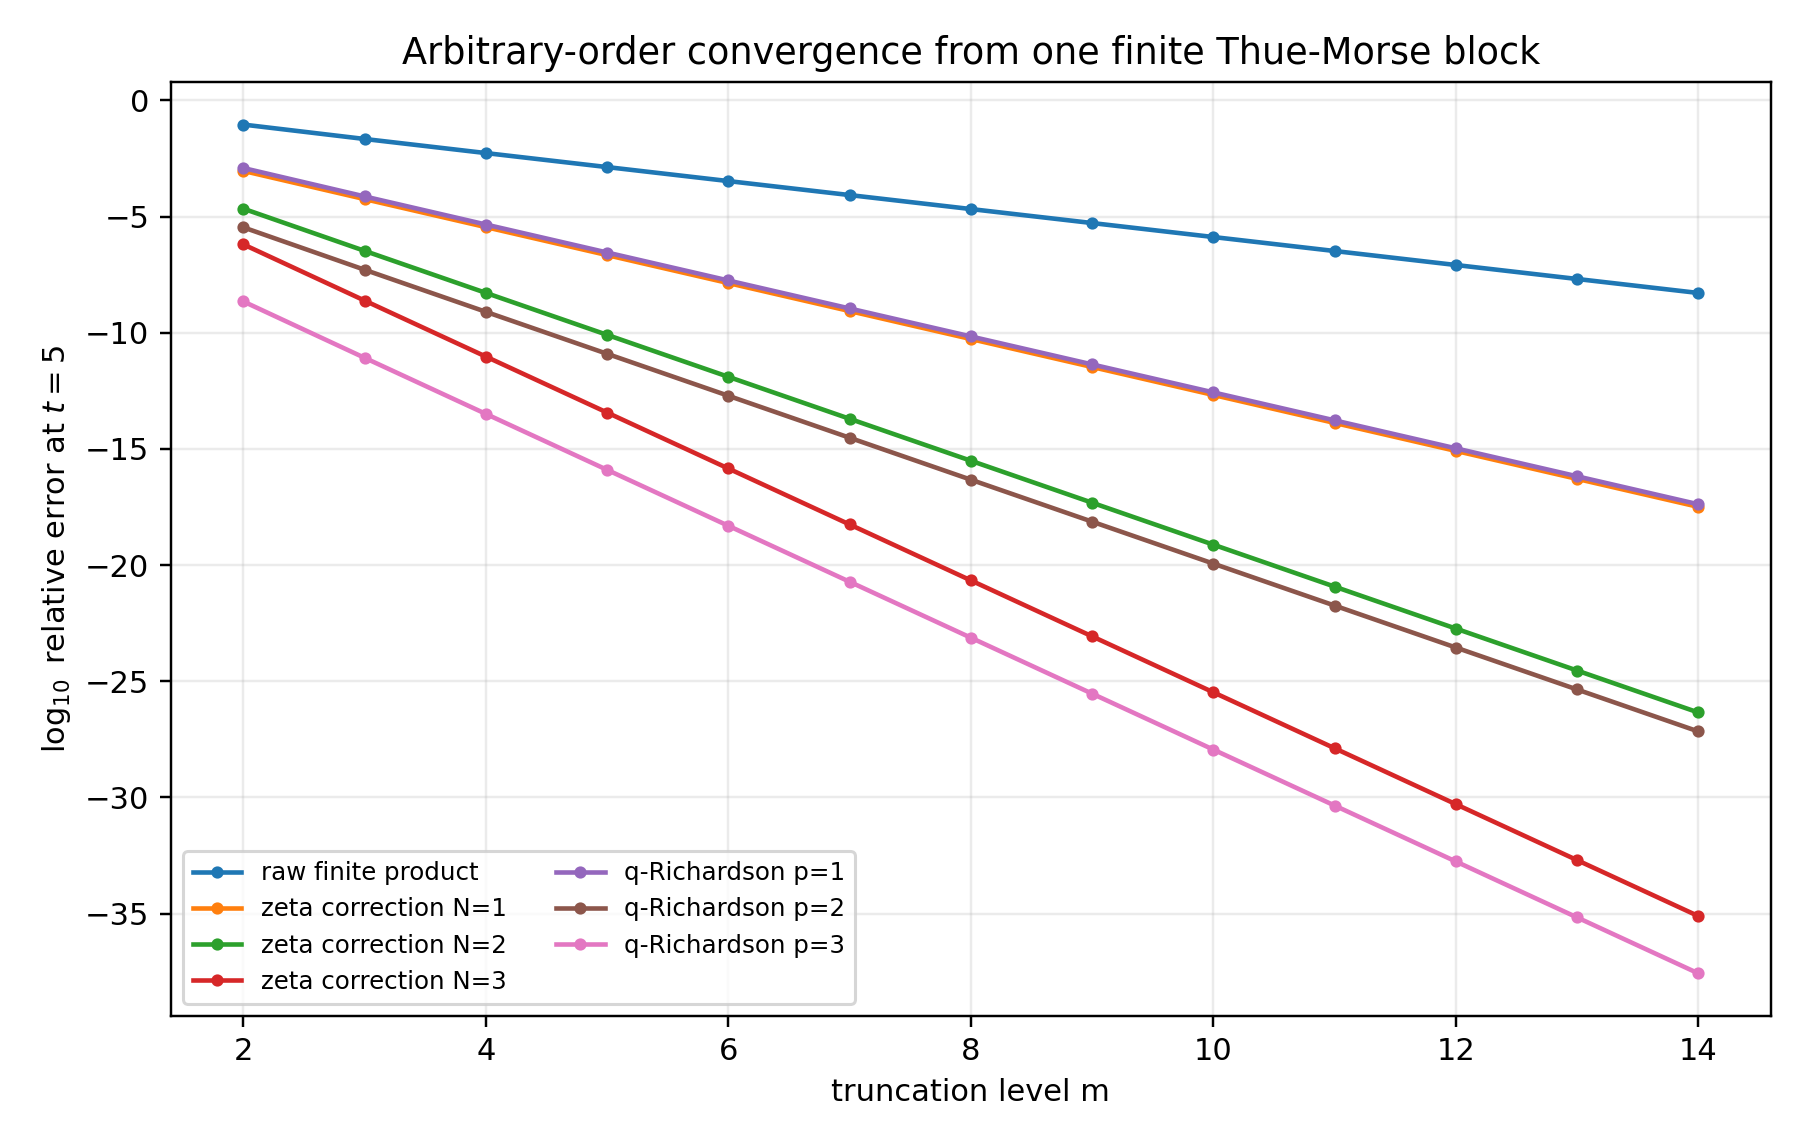
\includegraphics[width=0.97\textwidth]{figures/spectral_convergence.png}
\caption{Relative errors at $t=5$.  Every zeta correction or Richardson degree raises the
power of $4^{-m}$ by one, exactly as predicted by
\cref{cor:arbitrary-Q,thm:qRichardson}.}
\label{fig:spectral-convergence}
\end{figure}

A least-squares fit to the final five points of each curve gives:
\begin{center}
\small
\begin{tabular}{@{}lcc@{}}
\toprule
method & fitted order in $4^{-m}$ & proved order \\
\midrule
raw $Q_m$ & $1.00000013$ & $1$\\
zeta correction $N=1$ & $2.00000006$ & $2$\\
zeta correction $N=2$ & $3.00000007$ & $3$\\
zeta correction $N=3$ & $4.00000008$ & $4$\\
$q$-Richardson $p=1$ & $2.00000014$ & $2$\\
$q$-Richardson $p=2$ & $3.00000013$ & $3$\\
$q$-Richardson $p=3$ & $4.00000013$ & $4$\\
\bottomrule
\end{tabular}
\end{center}

\subsection{Weak expansion check}

For $\varphi(y)=\e^y$, all derivatives equal $\e^y$, so
\cref{thm:weak-expansion} becomes a direct moment correction to the finite moment-generating
function.  The relative errors are:
\begin{center}
\small
\begin{tabular}{@{}rcccc@{}}
\toprule
$m$ & raw spline & through $\mu_2$ & through $\mu_4$ & through $\mu_6$\\
\midrule
2 & $3.465\times10^{-3}$ & $4.569\times10^{-6}$ & $3.311\times10^{-9}$ & $1.540\times10^{-12}$\\
4 & $2.170\times10^{-4}$ & $1.789\times10^{-8}$ & $8.105\times10^{-13}$ & $2.357\times10^{-17}$\\
6 & $1.356\times10^{-5}$ & $6.991\times10^{-11}$ & $1.979\times10^{-16}$ & $3.597\times10^{-22}$\\
8 & $8.477\times10^{-7}$ & $2.731\times10^{-13}$ & $4.832\times10^{-20}$ & $5.489\times10^{-27}$\\
10 & $5.298\times10^{-8}$ & $1.067\times10^{-15}$ & $1.180\times10^{-23}$ & $8.375\times10^{-32}$\\
\bottomrule
\end{tabular}
\end{center}
Each added even moment raises the order by one power of $4^{-m}$.

\subsection{Endpoint-tail coefficients}

The absolute errors in approximating $\log G(-u)$ by the exact linear term plus the first
$N$ even corrections are:
\begin{center}
\small
\begin{tabular}{@{}rcccc@{}}
\toprule
$u$ & $N=0$ & $N=1$ & $N=2$ & $N=3$\\
\midrule
$0.02$ & $5.56\times10^{-6}$ & $3.70\times10^{-12}$ & $5.60\times10^{-18}$ & $1.04\times10^{-23}$\\
$0.2$ & $5.56\times10^{-4}$ & $3.70\times10^{-8}$ & $5.60\times10^{-12}$ & $1.04\times10^{-15}$\\
$1$ & $1.39\times10^{-2}$ & $2.31\times10^{-5}$ & $8.71\times10^{-8}$ & $4.03\times10^{-10}$\\
$3$ & $1.23\times10^{-1}$ & $1.81\times10^{-3}$ & $6.12\times10^{-5}$ & $2.54\times10^{-6}$\\
\bottomrule
\end{tabular}
\end{center}
The deterioration as $u$ approaches the exact radius $4\pi$ is governed by the certified
bound \eqref{eq:G-rem}.

\subsection{Lambert-depth experiment}

For $x=10^{-8}$,
\[
 \lambda(x)=31.555232088424067978\ldots,
 \qquad s_0(x)=3.1555232088424068\times10^9.
\]

\begin{figure}[htbp]
\centering
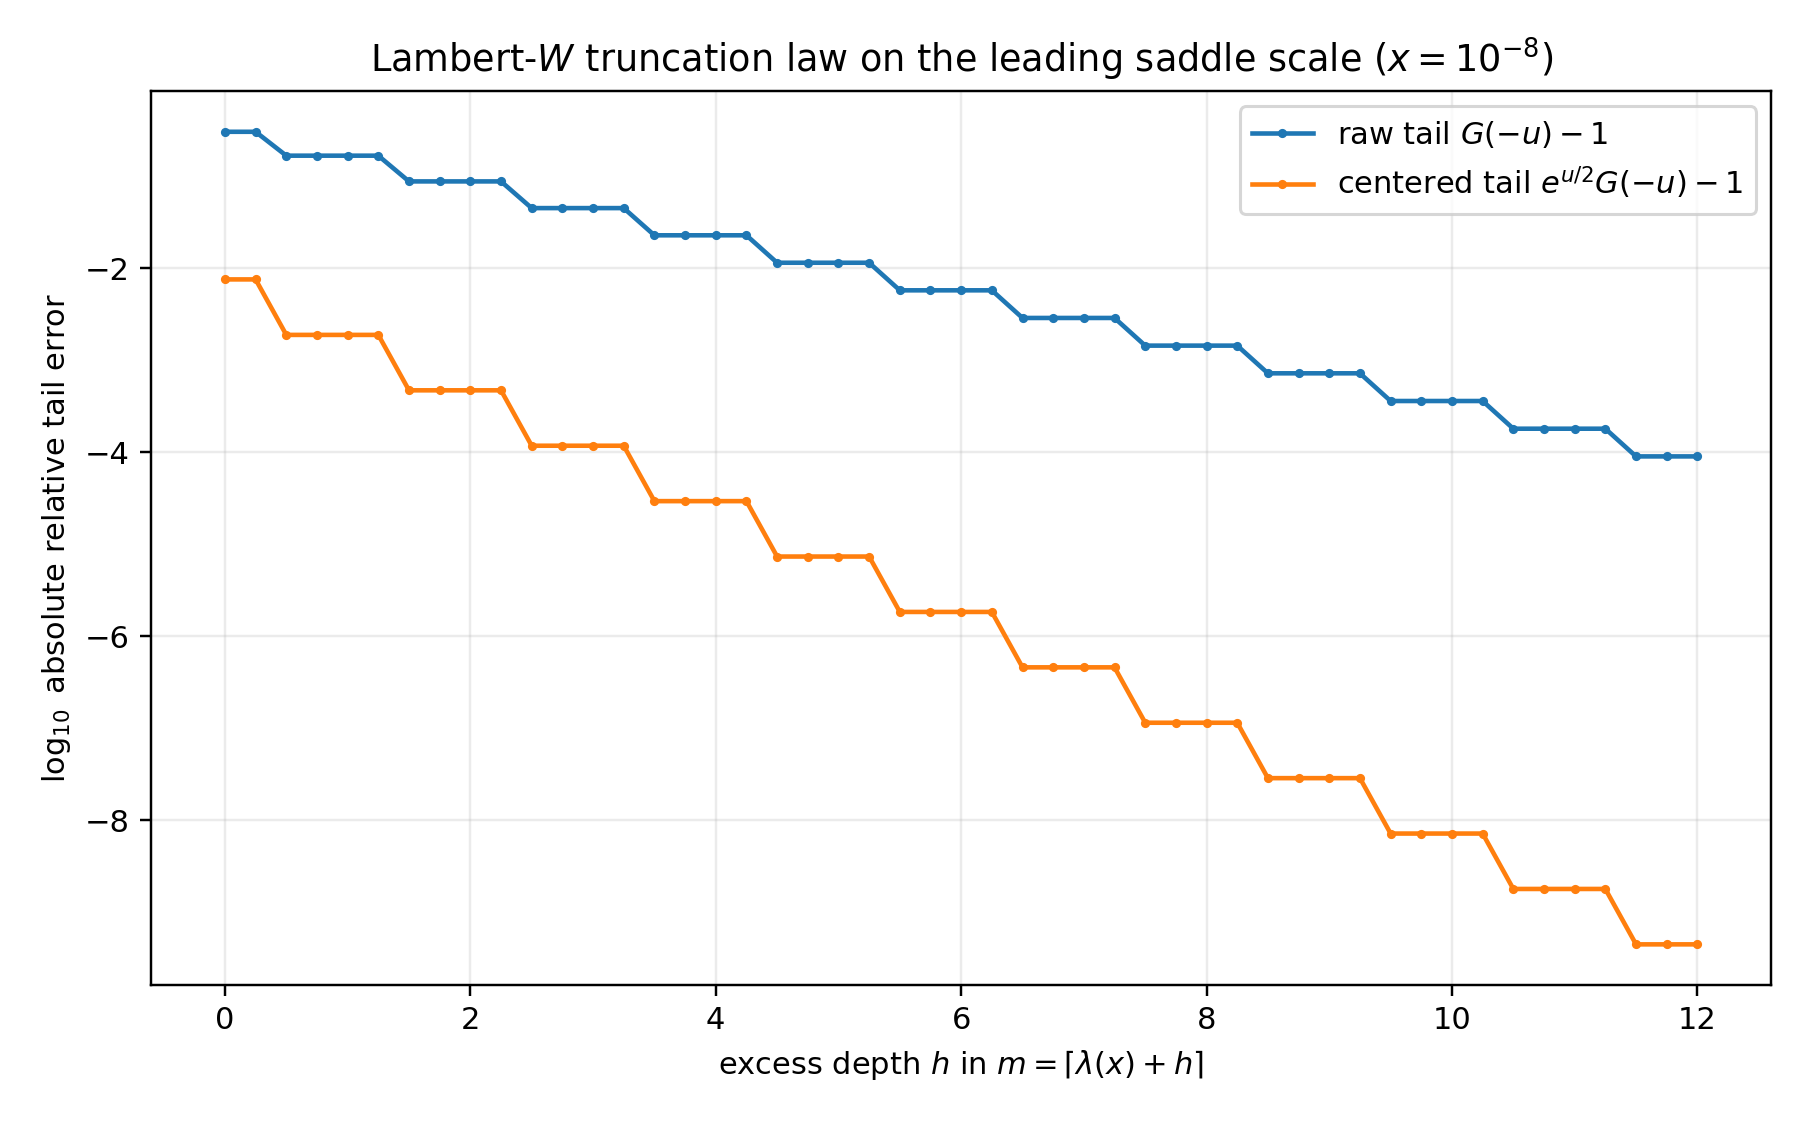
\includegraphics[width=0.97\textwidth]{figures/lambert_truncation.png}
\caption{Tail error when $m=\lceil\lambda(x)+h\rceil$.  Ceiling effects create the steps.
The raw tail gains about one binary digit per extra factor; the centered tail gains about two,
as proved in \cref{thm:depth-law}.}
\label{fig:Lambert-depth}
\end{figure}

At $h=8$, for example, $m=40$ and $u\approx2.8699\times10^{-3}$; the raw tail error is
$1.43\times10^{-3}$ while the centered tail error is $1.14\times10^{-7}$.

\clearpage
\section{Consequences for the existing research program}
\label{sec:consequences}

\subsection{A new exact-arithmetic/Fourier bridge}

The Atlas treats the block polynomial $P_m$ as a digital and algebraic object, while the
Fourier-decay program treats dyadic sinc products through shell dynamics and lacunary sine
products.  Theorem \ref{thm:finite-sinc} shows these are not merely related by analogy:
$P_m$ is the finite sinc product after one explicit normalization.  This provides a direct
translation dictionary:
\begin{center}
\small
\begin{tabular}{@{}ll@{}}
\toprule
finite digital statement & spectral statement \\
\midrule
order-$m$ zero of $P_m$ at $1$ & removable $t^{-m}$ normalization at the origin\\
Thue--Morse exponential sum & truncated up-function Fourier transform\\
Prouhet moment cancellation & high-order low-frequency cancellation\\
block length $2^m$ & product depth $m$\\
geometric error $4^{-m}$ & variance scale of omitted random tail\\
\bottomrule
\end{tabular}
\end{center}

The shell-factorization results remain essential for large real $t$ with $m$ tied to the
frequency shell.  The present tail calculus addresses a different regime: once the first
$m$ factors have been isolated, it computes the remaining small-argument factor to arbitrary
order.  The two analyses are complementary rather than competing.

\subsection{A new $q$-binomial role}

The repository's dyadic arithmetic naturally uses $q=1/2$ because scales and evaluation
points are dyadic.  The present extrapolation naturally uses $q=1/4$ because the centered
error expansion is even.  Gaussian binomials now appear in a second structural role:
\begin{equation}
 \text{exact dyadic values: }q=\frac12,
 \qquad
 \text{spectral-tail acceleration: }q=\frac14.
 \label{eq:two-q}
\end{equation}
This distinction is conceptually useful.  It prevents the $q$-binomial notation from being
viewed as an incidental encoding of one exact formula; it reflects two different geometric
lattices in the same theory.

\subsection{A certified route from finite splines to $\Up$}

The repeated-integration dossiers identify finite stages with compactly supported splines and
prove convergence.  The random-tail theorem strengthens the conceptual picture:
\[
 \text{limit law} = \text{finite spline law} + \text{scaled independent copy of the limit law}.
\]
The weak expansion \eqref{eq:weak-expansion} then supplies every correction coefficient and a
one-line remainder bound.  For numerical integration against smooth observables, the result
is immediately useful: one may integrate against the elementary finite spline $u_m$ and add
explicit derivative corrections, without ever sampling the limiting density directly.

\subsection{A product engine for endpoint saddles}

The endpoint theory's difficult part is the periodically modulated saddle, not the mere
existence of the product.  Nevertheless, every saddle evaluation repeatedly calls the
negative-Laplace product and its derivatives.  Formula \eqref{eq:G-TM-all} suggests a hybrid
implementation:
\begin{enumerate}
\item use the existing lower-Lambert phase and periodic saddle jets to choose $s$;
\item choose $m$ from the centered depth law \eqref{eq:mctr};
\item evaluate the exact finite Thue--Morse block and a few Bernoulli corrections;
\item differentiate the finite factorization rather than the infinite product.
\end{enumerate}
Because $u=s/2^m$ is small by construction, all differentiated correction series remain in a
controlled analytic disk.  This could turn the qualitative endpoint expansion into a
certified high-precision algorithm with transparent complexity.

\subsection{Formalization leverage}

The main new identities have unusually short dependency chains.  The finite bridges are
finite-product algebra.  Tail self-similarity is reindexing.  The weak expansion is Taylor's
theorem plus independence and symmetry.  The $q$-Richardson weights are finite Lagrange
interpolation.  Only the analytic logarithm and explicit zeta remainder require a substantial
complex-analysis layer.  This makes the package a plausible next formalization target --- and
in large part it is not a target at all but already done: as the \emph{Formal version}
paragraphs throughout \cref{sec:objects,sec:bridges,sec:zeta-tail,sec:richardson,sec:gamma-tower}
record, the block identity, both finite bridges in their unnormalized form, both halves of
tail self-similarity, the Fourier--Laplace rotation, the Lagrange characterization of the
$q$-Richardson weights with all three of its moment identities together with their closed
$q$-binomial form (compiled in \path{GeometricQBinomialLagrange.lean}), the $r=0$ layer
of the gamma tower, and now the entire zeta--Lambert tail calculus --- the Euler--zeta
logarithm, the all-orders expansion, the certified remainder, and the exact
prefix--corrections--tail split (\path{EulerLogTransform.lean}, \path{SincZetaSeries.lean},
\path{SincZetaDyadic.lean}, \path{SincZetaRemainder.lean}) --- already have Lean
counterparts, several of them more general than the statements printed here.  The weighted
Richardson remainder and the probabilistic layer are the remaining formalization targets.

\section{Lean formalization roadmap}
\label{sec:formalization}

The finite-block calculus has been deliberately organized so that the algebraic core can be
formalized before the analytic refinements.  The following dependency table separates the
short, high-confidence lemmas from the portions that require additions to the surrounding
analysis library.

Five of its rows have since been overtaken by the library --- two of them completely --- and
are retained because the table is also a dependency map.  The finite Thue--Morse product
\eqref{eq:Pm} is
\lean{Fabius.prod_one_sub_pow_eq_sum_thueMorseSign}, proved over an arbitrary commutative
ring, not by the coefficient induction suggested below.  The finite sinc bridge
\eqref{eq:finite-sinc} and the finite Laplace bridge \eqref{eq:finite-Laplace} exist as
\lean{Fabius.sum_thueMorseSign_exp_eq_sin_prod} and
\lean{Fabius.sum_range_two_pow_thueMorseSign_exp}, in each case for real argument and in the
form preceding the $\sinc$, respectively $2^{m(m+1)/2}s^{-m}$, normalization; what those rows
still describe accurately is the remaining work, namely the removable value at the origin and
the extension to complex argument.  Exact tail self-similarity
\eqref{eq:Q-tail-self}--\eqref{eq:G-tail-self} is fully discharged, and the reusable
reindexing lemma the row asks for is exactly what was proved:
\lean{Fabius.tprod_geom_scale_pow} is stated for an arbitrary function into a commutative
topological monoid.  Of the $q$-Richardson row, the interpolation characterization
\eqref{eq:weights-Lagrange} and the moment identities
\eqref{eq:moment-cancel}--\eqref{eq:first-uncancelled} are done over an arbitrary field and
arbitrary ratio; only the Gaussian-binomial normalization \eqref{eq:weights} remains.  The
remaining rows --- the Euler--zeta logarithm, the certified zeta remainder, the random-tail
law, the weak expansion, the Lambert depth law, and the levels $r\ge1$ of the gamma tower ---
have no formal counterpart at present, and the Euler--zeta logarithm is, as stated below,
still the pivot: it is what the remainder bound, the corrected approximants, the cumulant
formula and the base-$b$ theorem all reduce to.

\begingroup
\small
\setlength{\LTleft}{0pt}
\setlength{\LTright}{0pt}
\begin{longtable}{@{}p{0.20\textwidth}p{0.24\textwidth}p{0.50\textwidth}@{}}
\toprule
Target & Minimal ingredients & Suggested proof strategy and principal risk \\
\midrule
\endfirsthead
\toprule
Target & Minimal ingredients & Suggested proof strategy and principal risk \\
\midrule
\endhead
Finite Thue--Morse product
\eqref{eq:Pm} & finite products, binary recursion, geometric sums & Prove
$P_{m+1}(z)=P_m(z)(1-z^{2^m})$ and identify coefficients by induction.  This should be almost
entirely algebraic. \\
Finite sinc bridge
\eqref{eq:finite-sinc} & complex exponential identities, finite-product reindexing & Rewrite
$1-\e^{2\ii x}=-2\ii\e^{\ii x}\sin x$, then normalize powers of two.  The only nuisance is a
clean treatment of the removable value at $t=0$. \\
Finite Laplace bridge
\eqref{eq:finite-Laplace} & real or complex exponentials, finite products & Substitute
$z=\e^{-s/2^m}$ in the block product and reindex.  This is the simplest new theorem in the
package. \\
Exact tail self-similarity
\eqref{eq:Q-tail-self}--\eqref{eq:G-tail-self} & convergence of infinite products, shifted
indices & Establish a reusable infinite-product reindexing lemma.  Existing repository
convergence results should discharge the side conditions. \\
Euler--zeta logarithm
\eqref{eq:logsinc} & local analytic logarithm, Euler's sine product, normal convergence &
\emph{Delivered} in \path{SincZetaSeries.lean} (exponential and real-logarithm forms), on
the general Euler log transform of \path{EulerLogTransform.lean}; the all-orders identity
\eqref{eq:Q-all-orders} is \path{SincZetaDyadic.lean}. \\
Certified zeta remainder
\eqref{eq:Q-remainder-bound} & positivity, monotonicity of $\zeta(2r)$, geometric series &
\emph{Delivered} in \path{SincZetaRemainder.lean}: the verbatim bound, real-argument
nonnegativity, and the exact prefix--corrections--tail split. \\
$q$-Richardson weights
\eqref{eq:weights}--\eqref{eq:first-uncancelled} & finite Lagrange interpolation,
$q$-Pochhammer algebra & \emph{Delivered} in
\path{GeometricQBinomialLagrange.lean}: zero-extended numerator, reversed
denominator-free polynomial, normalized weight under node injectivity, and every positive
residual moment; \(q=1/2\) is linked to the Toeplitz row. \\
Random-tail law
\eqref{eq:random-tail} & independent random variables, almost-sure summation, equality in law &
Split and reindex the convergent random series.  A characteristic-function proof may be
shorter if the current probability library lacks convenient random-series infrastructure. \\
Weak expansion
\eqref{eq:weak-expansion} & Taylor theorem with remainder, expectation inequalities, symmetry &
Condition on the finite sum; use bounded support to make the remainder estimate immediate. \\
Lambert depth law
\eqref{eq:mraw}--\eqref{eq:mctr} & branch $W_{-1}$, ceilings, local exponential estimates & The
analytic estimate is elementary after the definition of $\lambda$; the likely missing piece is
a convenient formal API for the lower real Lambert branch. \\
Thue--Morse gamma tower
\eqref{eq:gamma-Mellin}--\eqref{eq:gamma-iterated} & holomorphic parameter differentiation,
reciprocal-gamma zero, Atlas Dirichlet continuation & Reuse the Atlas continuation theorem;
prove the simple-zero coefficient of $1/\Gamma$ at each nonpositive integer; then
differentiate the dyadic equation and the shift parameter identity. \\
\bottomrule
\end{longtable}
\endgroup

A practical promotion sequence is therefore
\[
 \boxed{\begin{gathered}
 \text{finite bridges}
 \longrightarrow \text{tail reindexing}
 \longrightarrow \text{probabilistic splitting}\\
 \longrightarrow \text{$q$-interpolation}
 \longrightarrow \text{analytic logarithms}
 \end{gathered}}
\]
The first four stages already yield exact identities and acceleration mechanisms.  The final
stage adds the sharp radius and explicit zeta remainder.  This ordering minimizes the amount
of new complex analysis that must be trusted at any one time.  Of the boxed chain, the
finite bridges, tail reindexing, $q$-interpolation, and analytic-logarithm stages are now
formal (see the \emph{Formal version} paragraphs above); the probabilistic splitting is the
one stage that remains.

\begin{obligation}[Canonical normalization theorem]
The repository uses several Fourier-transform conventions across historical manuscripts.
A promoted theorem should package the convention explicitly and derive all rescalings between
$F$, $\Up$, $Q_\infty$, and the characteristic function of $Y_\infty$.  Doing so would prevent
sign and $2\pi$ factors from leaking into later shell or saddle arguments.
\end{obligation}

This obligation stands, but part of the required chain is already formal and fixes the
convention unambiguously: \lean{Fabius.rvachevFourier} is
$\int_\R\Up(t)\e^{-2\pi\ii tz}\dd t$,
\lean{Fabius.rvachevFourier_eq_product} converts it into $Q_\infty$, and
\lean{Fabius.complexGeneratingFunction_eq_fourier_analytic} together with
\lean{Fabius.complexGeneratingFunction_neg_eq_tprod} carries the rotation to $G$.  What the
obligation still asks for is the remaining leg --- the $F\leftrightarrow\Up$ rescaling
\eqref{eq:Fup} and the characteristic function of $Y_\infty$ --- packaged with the others as a
single named normalization theorem rather than reconstructed at each use.

\begin{obligation}[Reusable geometric-tail API]
The identity ``tail equals a scaled copy of the whole object'' occurs simultaneously for
products, convolutions, random series, and cumulant generating functions.  A small abstract
library for geometrically self-similar tails would make the dyadic case a specialization
rather than four separate proofs.
\end{obligation}

The product quarter of this obligation is discharged.  \path{GeometricScaleProducts.lean}
is exactly the abstract library asked for on the product side:
\lean{Fabius.tprod_geom_scale} and \lean{Fabius.tprod_geom_scale_pow} are proved for an
arbitrary function from a field into a commutative topological monoid and an arbitrary scale,
with the dyadic sinc shells obtained as specializations, exactly as the obligation proposes.
The logarithmic face of the same abstraction is now \path{EulerLogTransform.lean}: the
transform $\sum_i\log(1-a_i)=-\sum_{r\ge1}\bigl(\sum_ia_i^r\bigr)/r$ for an arbitrary
absolutely summable family with every norm below one, over an arbitrary index type, with the
geometric family --- the self-similar tail par excellence --- as its first instance.
(The negative-Laplace tail \eqref{eq:G-tail-self} is formal too, but as an independent
induction on the functional equation rather than as an instance of that API --- which is
itself a small illustration of the duplication the obligation is about.)  The obligation is
retained because its other three instances ---
convolutions, random series, and cumulant generating functions, that is
\eqref{eq:density-deconv}, \eqref{eq:random-tail} and \eqref{eq:cumulant-operator} --- have no
formal counterpart, and because nothing yet expresses the four as instances of one statement.

\section{Frontier conjectures and next deductions}
\label{sec:frontiers}

The proved results isolate several questions which are both sharper and more tractable than
the broad open-ended prompts in the older frontier notebooks.  The statements below are
intentionally separated from the theorem package.

\begin{conjecture}[Certified endpoint evaluator with near-optimal product depth]
\label{conj:endpoint-evaluator}
There is a fully explicit algorithm which, for sufficiently small $x>0$ and target relative
error $\eta$, evaluates $F(x)$ using
\begin{equation}
 -\frac{W_{-1}(-x\log2)}{\log2}
 +\frac12\log_2\frac1\eta+\bigO(1)
 \label{eq:conj-depth}
\end{equation}
product layers, together with a bounded-order periodic saddle jet, and whose final error is
rigorously at most $\eta$.  The coefficient $1/2$ in the precision surcharge is optimal among
methods which first center the omitted product but do not cancel its quadratic cumulant.
\end{conjecture}

The depth estimate itself is proved in \cref{thm:depth-law}.  What remains is to propagate the
product error, its differentiated versions, and the periodic saddle displacement through the
complete inversion formula.  The conjectured optimality should follow from the nonzero
variance $\kappa_2=1/9$.

\begin{conjecture}[Cumulant-cancelled endpoint hierarchy]
\label{conj:cumulant-depth}
After removing the first $N$ even cumulants of the centered tail in addition to the linear
factor, the extra depth required for tolerance $\eta$ is
\begin{equation}
 \frac{1}{2N+2}\log_2\frac1\eta+\bigO_N(1).
 \label{eq:cumulant-depth-conj}
\end{equation}
Equivalently, the $N$-corrected finite block should require only one additional product layer
for every $2N+2$ requested binary digits of tail accuracy.
\end{conjecture}

This is already a theorem for the isolated product, by \eqref{eq:G-rem}; the conjectural part
is that the same saving survives uniformly through the full saddle inversion, including all
needed derivatives and the periodic phase.

\begin{conjecture}[Strong spline correction away from knots]
\label{conj:strong-spline}
Fix $N\ge0$ and a compact interval $K\subset(-1,1)$.  After excluding a neighborhood of the
knots of the finite spline $u_m$ whose width is comparable to $2^{-m}$, the distributional
expansion \eqref{eq:distributional} admits a pointwise or Hölder-norm version through order
$N$, with remainder $\bigO_K(4^{-(N+1)m})$ after the natural derivative scaling.
\end{conjecture}

A global pointwise statement cannot be obtained by naively differentiating $u_m$: finite
splines have knots, whereas $\Up$ is smooth.  The random-tail convolution indicates two viable
repairs.  One may either retain the exact final mollifier $2^m\Up(2^m\cdot)$, or state the
expansion on cells separated from their endpoints.  Establishing the best norm and boundary
layer is a concrete approximation-theoretic problem.

\begin{conjecture}[Dual-$q$ transmutation]
\label{conj:dual-q}
There is a direct coefficient-level transform taking a substantial class of the repository's
$q=1/2$ exact dyadic formulae into $q=1/4$ spectral-tail acceleration identities, with the
squaring $q\mapsto q^2$ explained by parity or centering rather than by an ad hoc substitution.
\end{conjecture}

Evidence is structural: the exact dyadic theory resolves single binary scales, while every
centered Fourier or probability correction is even and therefore sees squared scales.  A
useful form of the conjecture would turn Gaussian-binomial coefficient extraction at
$q=1/2$ into geometric-grid interpolation at $q=1/4$.

\begin{conjecture}[Automatic Barnes hierarchy]
\label{conj:automatic-Barnes}
The functions $\Gamma_r^{\rm TM}$ possess canonical Weierstrass products and asymptotic
normalizations for which the dyadic law \eqref{eq:gamma-dyadic} and differential ladder
\eqref{eq:gamma-differential} uniquely characterize the hierarchy, analogously to the role of
convexity or normalization in classical gamma-type characterizations.
\end{conjecture}

The Mellin formula gives positivity and complete-monotonicity information for suitable signed
derivatives, while the dyadic equation supplies an automatic analogue of a multiplication
formula.  The remaining difficulty is to choose a normalization that removes the freedom to
multiply by functions invisible to the differential recursion.

\subsection{General radix and nonuniform tails}

The base-$b$ theorem \eqref{eq:base-b} shows that the zeta--Lambert mechanism does not depend
on binary arithmetic.  What is special to base two is the simultaneous existence of the
Thue--Morse block polynomial, the simple two-branch functional equation, and the Fabius/up
probability model.  A next generalization is to replace the uniform summands by centered
compactly supported variables $X_k$ at scales $b^{-k}$.  If their common characteristic
function has a nonzero analytic germ at the origin, then
\[
 \log\frac{\Phi_\infty(t)}{\Phi_m(t)}
 =\sum_{r\ge1}c_r t^r\frac{b^{-r(m+1)}}{1-b^{-r}}.
\]
Thus Lambert kernels are universal for geometric random tails; the zeta values in the present
report are the special signature of the uniform law through Euler's sine product.  The
classification of digital substitutions whose finite block polynomial exactly realizes such
a characteristic product is a natural interface between automatic sequences and compactly
supported refinable laws.

\section{Conclusion}
\label{sec:conclusion}

The documentation corpus already supplied the large pieces: a careful separation of the
Fabius and up-function normalizations, an exact dyadic arithmetic theory rich in
$q$-binomial coefficients, a probabilistic convolution model, a detailed analysis of the
infinite sinc product, corrected lower-Lambert endpoint asymptotics, and a broad Thue--Morse
formula atlas.  The missing junction was finite-block calculus.

One polynomial now connects the principal domains:
\[
 \boxed{
 \begin{array}{c}
 P_m(z)=\displaystyle\sum_{n<2^m}\eps_nz^n\\[0.3em]
 \rotatebox{90}{$=$}
 \end{array}
 \quad
 \begin{array}{c}
 \text{finite digital block}\\
 \text{finite Fourier sinc product}\\
 \text{finite negative-Laplace product}
 \end{array}}
\]
after explicit phase and scale normalizations.  The omitted object is always a scaled copy of
the full object.  That observation produces exact all-order tails, zeta--Lambert coefficients,
Gaussian-binomial extrapolation, random-tail deconvolution, and Lambert-$W$ complexity laws
from a common source rather than as isolated formulas.

The principal proved advances are:
\begin{enumerate}
\item exact oscillatory and decaying substitutions converting a length-$2^m$ Thue--Morse block
      into the first $m$ factors of the Fourier and endpoint products;
\item a convergent all-orders logarithmic tail with exact radius and an explicit geometric
      remainder bound;
\item arbitrary-order corrected finite-block approximants and a separate $q$-Richardson
      scheme whose weights are Gaussian binomials at $q=1/4$;
\item an exact independent-copy decomposition of the omitted random tail, yielding a certified
      weak differential expansion of the up-law in finite uniform splines;
\item raw, centered, and higher-correction product-depth laws on the canonical lower-Lambert
      saddle scale;
\item a Thue--Morse gamma tower obtained by differentiating the entire shifted Dirichlet
      function at its trivial zeros.
\end{enumerate}

These results do not replace the repository's sharp shell dynamics or periodically modulated
endpoint saddle.  They add a complementary local engine: after a finite block or finite shell
has been isolated, the remainder is computable to arbitrary order with transparent constants.
That engine is algebraically short, numerically stable after centering, and unusually suitable
for formal verification.

\appendix
\clearpage
\section{Coefficient and extrapolation tables}
\label{app:coefficients}

\subsection{Zeta--Lambert and centered Laplace coefficients}

Write
\[
 a_r=\frac{\zeta(2r)}{r\pi^{2r}(4^r-1)},
 \qquad
 c_r=\frac{B_{2r}}{2r(2r)!(4^r-1)}.
\]
Then
\[
 \log\frac{Q_\infty(t)}{Q_m(t)}=-\sum_{r\ge1}a_rt^{2r}4^{-rm},
 \qquad
 \log C(-u)=\sum_{r\ge1}c_ru^{2r}.
\]
The first eight exact coefficients are:
\begin{center}
\small
\begin{tabular}{@{}rll@{}}
\toprule
$r$ & $a_r$ & $c_r$\\
\midrule
1 & $1/18$ & $1/72$\\
2 & $1/2700$ & $-1/43200$\\
3 & $1/178605$ & $1/11430720$\\
4 & $1/9639000$ & $-1/2467584000$\\
5 & $1/478533825$ & $1/490018636800$\\
6 & $691/15688261338750$ & $-691/64259118443520000$\\
7 & $2/2092151286225$ & $1/17138903336755200$\\
8 & $3617/170727360353550000$ & $-3617/11188788288130252800000$\\
\bottomrule
\end{tabular}
\end{center}
The numerators $691$ and $3617$ are the familiar Bernoulli numerators; here they enter through
the uniform-tail cumulants rather than through an independent number-theoretic construction.

\subsection{Analytic error germ}

For
\[
 H_t(r)=\frac1{Q_\infty(t\sqrt r)}=\sum_{n\ge0}h_n(t)r^n,
\]
the first coefficients are monomials in $t^2$:
\begin{align*}
 h_0(t)&=1,\\
 h_1(t)&=\frac{t^2}{18},\\
 h_2(t)&=\frac{31t^4}{16200},\\
 h_3(t)&=\frac{2347t^6}{42865200},\\
 h_4(t)&=\frac{1904369t^8}{1311675120000},\\
 h_5(t)&=\frac{3309760579t^{10}}{88561680752160000}.
\end{align*}
They are complete exponential Bell polynomials in $a_1t^2,a_2t^4,\ldots$.  Consequently,
all leading constants in \eqref{eq:Richardson-leading} are exact rational multiples of
$Q_\infty(t)t^{2p+2}$.

\subsection{Gaussian-binomial extrapolation weights}

At $q=1/4$, the first six rows are:
\begin{align*}
 p=0:&\quad (1),\\
 p=1:&\quad \left(-\frac13,\frac43\right),\\
 p=2:&\quad \left(\frac1{45},-\frac49,\frac{64}{45}\right),\\
 p=3:&\quad \left(-\frac1{2835},\frac4{135},-\frac{64}{135},
                         \frac{4096}{2835}\right),\\
 p=4:&\quad \left(\frac1{722925},-\frac4{8505},\frac{64}{2025},
                         -\frac{4096}{8505},\frac{1048576}{722925}\right),\\
 p=5:&\quad \left(-\frac1{739552275},\frac4{2168775},-\frac{64}{127575},
                         \frac{4096}{127575},-\frac{1048576}{2168775},
                         \frac{1073741824}{739552275}\right).
\end{align*}
The alternating signs are unavoidable because the formula extrapolates from positive nodes
$q^m,\ldots,q^{m+p}$ to the endpoint $0$.  For numerical work at very high $p$, barycentric or
compensated summation should be used rather than forming the rational coefficients in floating
point.

\section{Reproducibility protocol}
\label{app:reproducibility}

The numerical checks used direct high-precision arithmetic and did not fit coefficients that
were subsequently inserted into proofs.  The following pseudocode records the independent
verification path.

\begin{lstlisting}[style=pseudo,language=Python,caption={Independent verification skeleton}]
set_precision(100)

def epsilon(n):
    return (-1) ** binary_digit_sum(n)

def P(m, z):
    return product(1 - z ** (2 ** j) for j in range(m))

def Q_finite(m, t):
    return product(sinc(t / (2 ** k)) for k in range(1, m + 1))

def Q_infinite(t, cutoff):
    return product(sinc(t / (2 ** k)) for k in range(1, cutoff + 1))

# Exact finite identities
for (m, t) in test_grid:
    lhs = P(m, exp(1j * t / (2 ** (m - 1))))
    rhs = ((-1j) ** m * t ** m * 2 ** (-m * (m - 1) / 2)
           * exp(1j * t * (1 - 2 ** (-m))) * Q_finite(m, t))
    report(relative_residual(lhs, rhs))

# All-order tail and q-Richardson slopes
for m in depth_grid:
    exact = Q_infinite(t, large_cutoff)
    for N in correction_orders:
        approx = Q_finite(m, t) * exp(-sum(a(r) * t ** (2*r)
                                               * 4 ** (-r*m)
                                               for r in range(1, N + 1)))
        save_error(m, N, relative_error(approx, exact))
    for p in extrapolation_orders:
        approx = sum(weight(p, j) * Q_finite(m + j, t)
                     for j in range(p + 1))
        save_error(m, p, relative_error(approx, exact))
fit_final_log_slopes()

# Random-tail weak expansion, phi(y)=exp(y)
for m in depth_grid:
    finite_mgf = product(sinh(2 ** (-k)) / (2 ** (-k))
                         for k in range(1, m + 1))
    corrected = finite_mgf * sum(moment(2*j) * 4 ** (-j*m)
                                 / factorial(2*j) for j in range(N + 1))
    compare_with_infinite_mgf(corrected)
\end{lstlisting}

The oscillatory and Laplace finite identities were tested at levels up to $m=12$ with relative
residuals between $10^{-96}$ and $10^{-102}$.  Regression was used only to diagnose the
convergence exponent after the formulas had been proved; the fitted base-$4$ orders were
$1,2,3,4$ to roughly seven significant digits for the raw, first-, second-, and third-order
schemes.  The figures embedded in this report were generated from the same data.

\section{Complete corpus ledger and deduplication map}
\label{app:ledger}

\subsection{Living documentation treated as authoritative}

The audit covered every TeX manuscript in the living documentation tree.  At the snapshot date,
the principal paths and roles were:

\begin{longtable}{@{}p{0.42\textwidth}p{0.52\textwidth}@{}}
\toprule
Path or group & Role in the audit\\
\midrule
\endfirsthead
\toprule
Path or group & Role in the audit\\
\midrule
\endhead
\path{Fabius_Function_and_Rvachev_Up/Fabius_Function_and_Rvachev_Up.tex}
& Primary synthesis: normalization, probability, Fourier theory, exact dyadic values, and
corrected endpoint asymptotics.\\
\path{FabiusFunction_Mathematical_Glossary/FabiusFunction_Mathematical_Glossary.tex}
& Terminology and notation cross-check.\\
\path{Non_Elementarity_of_the_Fabius_Function/Non_Elementarity_of_the_Fabius_Function.tex}
& Differential-algebraic and non-elementarity context.\\
\path{fabius_lean_walkthrough/fabius_lean_walkthrough.tex}
& Map between human mathematics, Lean files, dependencies, and proof status.\\
\path{non-formalized-research-frontiers/non-formalized-research-frontiers.tex}
& Consolidated gap register and non-formalized frontier synthesis.\\
\path{non-formalized-research-frontiers/drafts/Thue_Morse_Formula_Atlas/Thue_Morse_Formula_Atlas.tex}
& Current comprehensive formula atlas; principal source for the block polynomial and shifted
Dirichlet continuation.\\
\path{non-formalized-research-frontiers/drafts/rvachev_up_fourier_decay/}
& Twelve active manuscripts: the initial wave, comparative and second-wave audits, a gentle
guide, the asymptotic-product problem statement, successive waves 2--8, and the final
resolution.  They were compared rather than collapsed because their hypotheses and correction
histories differ.\\
\path{papers/AIF_76_21-38/}
& Original and corrected TeX transcriptions of Arias de Reyna's compact-support paper.\\
\path{papers/arXiv-1502.06738/}
& Source TeX for Aistleitner--Hofer--Larcher on parametric Thue--Morse sequences and lacunary
trigonometric products.\\
\path{papers/arXiv-1702.05442/}
& Source TeX for Arias de Reyna's English translation of the 1982 compact-support article.\\
\path{papers/arXiv-1702.06487/}
& Source TeX for Arias de Reyna's arithmetic study of dyadic Fabius values.\\
\path{papers/arXiv-2211.13570/}
& Source TeX for Tóth's shifted and combined Thue--Morse Dirichlet series.\\
\path{papers/ubiq15/ubiq15-corrected.tex}
& Corrected source for imported automatic-sequence background.\\
\bottomrule
\end{longtable}

Within the Fourier-decay group, the inspected subdirectories were
\path{Rvachev_Up_Fourier_Decay-2},
\path{Rvachev_Up_Fourier_Decay-3},
\path{Comparative_Audit},
\path{Gentle_Guide},
\path{Second_Wave_Audit},
\path{asymptotic-decay-rate-of-an-infinite-product-of-sinc-functions},
\path{rvachev_up_fourier_decay-1}, and
\path{rvachev_up_fourier_decay-4} through
\path{rvachev_up_fourier_decay-8}.  Each contains one principal TeX manuscript.

\subsection{Frozen archive represented through provenance}

The archive README states that entries preserve the first-introduced historical document,
that later edits are not separately archived, and that byte-identical copies already present
in the living tree were pruned.  Accordingly, the audit used the following unique historical
entries as a provenance map rather than counting every renamed or duplicated copy as new
mathematical evidence.

\begin{longtable}{@{}p{0.19\textwidth}p{0.75\textwidth}@{}}
\toprule
Archive category & Frozen entries\\
\midrule
\endfirsthead
\toprule
Archive category & Frozen entries\\
\midrule
\endhead
Early notes
& \path{Fabius Asymptotic};
  \path{K-fold summation over the signed Thue-Morse sequence}.\\
Standalone studies
& \path{Non_Elementarity_of_the_Fabius_Function};
  \path{Small_Argument_Asymptotics};
  \path{fabius-inverse-dyadic-closed-form}.\\
Primary exposition
& \path{Fabius_Function_and_Rvachev_Up};
  \path{Fabius_Function_and_Rvachev_Up-2};
  \path{Fabius_Function_and_Rvachev_Up-3};
  \path{Fabius_and_Rvachev_Up-2};
  \path{Fabius_and_Rvachev_up};
  \path{Fabius_function_and_up_function}.\\
Primary supplements
& \path{Fabius_Function_Missing_Parts};
  \path{Fabius_Function_Missing_Parts-2}.\\
$q$-calculus
& \path{Fabius_q_Special_Functions};
  \path{fabius-q-special-functions}.\\
Lean walkthrough
& Two frozen walkthrough variants recorded under the archive's
  \path{lean-walkthrough} category.\\
Glossary
& Two frozen glossary variants recorded under the archive's \path{glossary} category.\\
Research frontiers
& \path{Fabius_Dyadic_Asymptotic_Bridge};
  \path{Fabius_Dyadic_Formulae_and_Alternative_Representations};
  \path{Fabius_Dyadic_Formulae_to_Asymptotics};
  \path{Fabius_Dyadic_q_Connections};
  \path{Fabius_Thue_Morse_Convergence_Rate};
  \path{Fabius_Thue_Morse_Convergence_Rates};
  \path{Primary_Exposition_Gap_Register};
  \path{Repeated_Integration_and_Rvachev_Up};
  \path{Rvachev_Up_from_Repeated_Integration};
  \path{non-formalized-research-frontiers};
  \path{Thue_Morse_Formula_Atlas-1};
  \path{Thue_Morse_Formula_Atlas-2};
  \path{Thue_Morse_Formula_Atlas-3}.\\
\bottomrule
\end{longtable}

This ledger explains the phrase ``all TeX documents'' operationally: every living manuscript
was inspected, every active mutually auditing draft was retained, every imported TeX paper was
included, and frozen historical variants were read through their explicit provenance and
content map so that superseded copies did not distort novelty checks.

\begin{thebibliography}{99}

\bibitem{proveit-primary}
V.~Reshetnikov,
\emph{The Fabius Function and Rvachev's Up-Function: Exact arithmetic, probability, Fourier
analysis, and corrected sharp asymptotics}, living repository manuscript, 2026.
\url{https://github.com/VladimirReshetnikov/ProveIt/blob/main/Analysis/FabiusFunction/docs/Fabius_Function_and_Rvachev_Up/Fabius_Function_and_Rvachev_Up.tex}

\bibitem{proveit-frontiers}
V.~Reshetnikov,
\emph{Non-Formalized Research Frontiers for the Fabius Function}, living repository
manuscript, 2026.
\url{https://github.com/VladimirReshetnikov/ProveIt/blob/main/Analysis/FabiusFunction/docs/non-formalized-research-frontiers/non-formalized-research-frontiers.tex}

\bibitem{proveit-atlas}
V.~Reshetnikov,
\emph{A Unified Formula Atlas for the Thue--Morse Sequence}, living repository manuscript,
2026.
\url{https://github.com/VladimirReshetnikov/ProveIt/blob/main/Analysis/FabiusFunction/docs/non-formalized-research-frontiers/drafts/Thue_Morse_Formula_Atlas/Thue_Morse_Formula_Atlas.tex}

\bibitem{proveit-fourier}
V.~Reshetnikov,
\emph{The Fourier Decay of Rvachev's Up-Function: Final Resolution}, living repository
manuscript, 2026.
\url{https://github.com/VladimirReshetnikov/ProveIt/blob/main/Analysis/FabiusFunction/docs/non-formalized-research-frontiers/drafts/rvachev_up_fourier_decay/rvachev_up_fourier_decay-5/Rvachev_Up_Fourier_Decay_Final.tex}

\bibitem{proveit-archive}
V.~Reshetnikov,
\emph{Archive of historical document versions}, provenance README, 2026.
\url{https://github.com/VladimirReshetnikov/ProveIt/tree/main/Analysis/FabiusFunction/docs/archive}

\bibitem{arias1982}
J.~Arias de Reyna,
\emph{An infinitely differentiable function with compact support: Definition and properties},
English translation of \emph{Definici\'on y estudio de una funci\'on indefinidamente
diferenciable de soporte compacto}, Rev. Real Acad. Ciencias Madrid \textbf{76} (1982),
21--38; arXiv:1702.05442 (2017).
\url{https://arxiv.org/abs/1702.05442}

\bibitem{arias2017arith}
J.~Arias de Reyna,
\emph{Arithmetic of the Fabius function}, arXiv:1702.06487v3 (2017).
\url{https://arxiv.org/abs/1702.06487}

\bibitem{aistleitner2015}
C.~Aistleitner, R.~Hofer, and G.~Larcher,
\emph{On parametric Thue--Morse sequences and lacunary trigonometric products},
arXiv:1502.06738v2 (2015).
\url{https://arxiv.org/abs/1502.06738}

\bibitem{toth2022}
L.~T\'oth,
\emph{Linear Combinations of Dirichlet Series Associated with the Thue--Morse Sequence},
INTEGERS \textbf{22} (2022), Article 98; arXiv:2211.13570.
\url{https://arxiv.org/abs/2211.13570}

\bibitem{corless1996}
R.~M. Corless, G.~H. Gonnet, D.~E.~G. Hare, D.~J. Jeffrey, and D.~E. Knuth,
\emph{On the Lambert $W$ function}, Advances in Computational Mathematics \textbf{5} (1996),
329--359.
\url{https://doi.org/10.1007/BF02124750}

\bibitem{allouche2003}
J.-P. Allouche and J.~Shallit,
\emph{Automatic Sequences: Theory, Applications, Generalizations}, Cambridge University
Press, 2003.

\end{thebibliography}

\end{document}
